%
% ACPR 2015 template adaptation
%! TEX root = master.tex
\documentclass[10pt,twocolumn,letterpaper, 
]{article}
%\title{Control Methods of a muscular force model including muscular fatigue}

%% Latex documents that need direct input
%
% ACPR template packages
\usepackage{acpr}
\usepackage{times}
\usepackage{acro}
\usepackage{epsfig}
\usepackage{amsmath}
\usepackage{amssymb}
\acresetall
%  The following command loads a graphics package to include images
%  in the document. It may be necessary to specify a DVI driver option,
%  e.g., [dvips], but that may be inappropriate for some LaTeX
%  installations.
\usepackage[]{graphicx}

% In order to include files without having a clear page using \include*,
% the newclude package is required
\usepackage{newclude}

% Required for acronyms
%use \acresetall to reset the acroyms counter
%macros=True, allows for calling \myTriger rather than \ac{myTriger}
%\usepackage[single=true, macros=true, xspace=true]{acro}

% Use biblatex to manage the referencing
%
\usepackage[style=ieee, backend=biber, backref=true]{biblatex}

% Include other packages here, before hyperref.

% If you comment hyperref and then uncomment it, you should delete
% egpaper.aux before re-running latex.  (Or just hit 'q' on the first latex
% run, let it finish, and you should be clear).
\usepackage[%pagebackref=true,
            breaklinks=true,
            letterpaper=true,
            colorlinks,
            bookmarks=false,
           ]{hyperref}

% Clever cross referencing. Using cleverref, instead of writting
% figure~\ref{...} or equation~\ref{...}, only \cref{...} is required.
% The package interprates the references and introduces the figure, fig.,
% equation, eq., etc keywords. \Cref forces first letter capital.
% >> WARNING: This package needs to be loaded after hyperref, math packages,
%             etc. if used.
%             Cleveref is recomended to load late
\usepackage{cleveref}

% To create random text use lipsum
\usepackage{lipsum}
%\usepackage{translations}        % contains the latex packages
\title{Tackling the Curse of Data Imbalancing for Melanoma Classification}

\author{Mojdeh Rastgoo, Guillaume Lema\^itre, Rafael Garcia\\
Universitat de Girona\\
Campus Montilivi, Edifici P4, 17071 Girona\\
% For a paper whose authors are all at the same institution,
% omit the following lines up until the closing ``}''.
% Additional authors and addresses can be added with ``\and'',
% just like the second author.
% To save space, use either the email address or home page, not both
\and
Joan Massich, Olivier Morel, Fabrice M\'eriaudeau, Franck Marzani\\
Universit\'e de Bourgogne Franche-Comt\'e\\
12 rue de la Fonderie, 71200 Le Creusot\\
}
             % contains the Title and Autor info
%%%%%%%%%%%%%%%%%%%%%%%%%%%%%%%%%%%%%%%%%%%%%%%%%%%%%%%%%%%%% 
%>>>> uncomment following for page numbers
% \pagestyle{plain}    
%>>>> uncomment following to start page numbering at 301 
%\setcounter{page}{301} 
      % contains package and variables init.
%% Acronym definition example using glossaries package
%% \usepackage{acro} is required
%% 
%% For a powerful usage of the acro package look at http://tex.stackexchange.com/questions/135975/how-to-define-an-acronym-by-using-other-acronym-and-print-the-abbreviations-toge

\DeclareAcronym{cnn}{
  short = CNN,
  long = Condensed Nearest Neighbour
}

\DeclareAcronym{nn}{
  short = NN,
  long = Nearest Neighbour
}

\DeclareAcronym{oss}{
  short = OSS,
  long = One-Sided Selection
}

\DeclareAcronym{smote}{
  short = SMOTE,
  long = Synthetic Minority Over-sampling TEchnique
}

\DeclareAcronym{enn}{
  short = ENN,
  long = Edited Nearest Neighbour
}

\DeclareAcronym{svm}{
  short = SVM,
  long = Support Vector Machines
}

\DeclareAcronym{cad}{
  short = CAD, 
  long = Computer-Aided Diagnosis
}

\DeclareAcronym{clbp}{
  short = CLBP,
  long = Completed Local Binary Pattern
}
\DeclareAcronym{lbp}{
  short = LBP,
  long = Local Binary Pattern
}
\DeclareAcronym{rf}{
  short = RF,
  long = Random Forests
}

\DeclareAcronym{ncr}{
  short = NCR,
  long = Neighborhood Cleaning Rule
}

\DeclareAcronym{se}{
  short = SE,
  long = Sensitivity
}

\DeclareAcronym{sp}{
  short = SP,
  long =  Specificity
}

\DeclareAcronym{wracc}{
  short = WRacc,
  long = Weighted Relative Accuracy
}

\DeclareAcronym{fpr}{
  short = FPR,
  long = False Positive Rate
}

\DeclareAcronym{nm}{
  short = NM,
  long = NearMiss
}

\DeclareAcronym{nm1}{
  short = NM1,
  long = NearMiss-1
}

\DeclareAcronym{nm2}{
  short = NM2,
  long = NearMiss-2
}

\DeclareAcronym{nm3}{
  short = NM3,
  long = NearMiss-3
}

\DeclareAcronym{os}{
  short = OS,
  long = Over-Sampling
}

\DeclareAcronym{ros}{
  short = ROS,
  long = Random Over-Sampling
}

\DeclareAcronym{us}{
  short = US,
  long = Under-Sampling
}

\DeclareAcronym{rus}{
  short = RUS,
  long = Random Under-Sampling
}

\DeclareAcronym{cus}{
  short = CUS,
  long = Clustering Under-Sampling
}

\DeclareAcronym{bd}{
  short = BD,
  long = Barrel Deformation
}

\DeclareAcronym{rdgm}{
  short = RDGM,
  long = Random Deformation using Gaussian Motion 
}

\DeclareAcronym{tl}{
  short = TL,
  long = Tomek Link 
}      % contains the acronims
%%%%%%%%%%%%%%attention enlever pour le final

\acprfinalcopy % *** Uncomment this line for the final submission
%%%%%%%%%%%%%%%

\def\acprPaperID{} % *** Enter the acpr Paper ID here
\def\httilde{\mbox{\tt\raisebox{-.5ex}{\symbol{126}}}}

% Pages are numbered in submission mode, and unnumbered in camera-ready
\ifacprfinal\pagestyle{empty}\fi

%%% Select inputing only one part of the document
%%\includeonly{content/intro/intro}   % the file wihtout .tex
%%\includeonly{content/other/other_content}
%%\includeonly{./content/acpr/example_content}
%
\addbibresource{./content/lit_review.bib}
\addbibresource{./content/biblatex-examples.bib}
\addbibresource{./content/egbib.bib}

\begin{document}
%\documentclass[letterpaper, 10 pt, conference]{ieeeconf} 
%\usepackage{graphicx} 
%\usepackage{amsmath}
%\usepackage{amssymb} 

\maketitle
\begin{abstract}

Electromyostimulation has been used for several decades by athletes or physiotherapists in order to create a muscular reinforcement. However, the efficiency of electromyostimulation is limited by muscular fatigue and by induced pain. Currently, the systems of electromyostimulation do not adapt the stimulation parameters automatically by taking into account physiological parameters such as muscular fatigue. To adapt the stimulation parameters to muscular responses and in order to optimize the rehabilitation sessions, a control of force using an indicator of muscular fatigue could be used. In this paper, we propose three ways to control the force by using a physiological model which includes the effects of muscular fatigue.
\end{abstract}
\section{Introduction}

The electromyostimulation (EMS) consists on sending electrical pulses through muscle with electrodes placed on the skin. These pulses induce muscular contractions without any brain command. Several works tried to model the effect of the stimulation on the developed force and the induced fatigue in a muscle. This task is a very important challenge because of the physiological differences between the different subjects (people) implies changes of model for each of them as in [1].

Even if experience based models are realized with a particular protocol, the set of equations developed in [2, 3] expresses, with a good accuracy the relation between parameters linking the force and the fatigue levels. Such a model is used to maximize the force and to reduce the muscular fatigue by predicting the necessary muscular contraction number (necessary frequency) analyzing the relation between the physiological aspects and the mathematical model [4]. The same model was studied in [5], the found EMS parameter, minimizing the fatigue, leads to a loss of generated force which can decrease down to 40\% of its maximal capability. Other studies based on the same model were realized in order to estimate the relation between the stimulation frequency and the force. Then, this relation correlate the effect of the stimulation frequency on the force and the fatigue rates [6, 7]. The previous model has already been used on children suffering of cerebral paralysis (CP) [8] to predict their muscular force. 

Currently, studies propose to control the torque of muscle, instead of the generated force, with a compensation of the force loss due to the fatigue apparition. Unlike the mentioned works, we propose some methods to control the force level during an EMS taking in account the muscular fatigue. We use the model proposed in [3, 4] with the aim to maintain the developed force of a muscle at a chosen reference force, despite of the apparition of the muscular fatigue. In this model, the control variable will be the inter pulse time which is linked to the induced force of the contraction. 
In the following, equations of the model are detailed. Then two control strategies are proposed in the case of the partial model (without fatigue) and the complete model. A set of simulations will be used to discuss about the control efficiency in a conclusion.

\section{Model}
The model is composed of two sub models: a force model (I) and a fatigue model (II) which includes the effects of the fatigue on the force level. The model (I) is defined by two differential equations:
\begin{equation}
\frac{dC_n}{dt}=\frac{1}{T_c}\sum R_ie^{\frac{-(t-t_i)}{T_c}}-\frac{C_n}{T_c}  ,
\end{equation}
\begin{equation}
	\frac{dF}{dt}=A\frac{C_n}{K_m+C_n}-\frac{F}{T_1+T_2(\frac{C_n}{K_m+C_n})}  ,
\end{equation}
with
\begin{equation}
R_i=1+(R_0-1)e^{-(\frac{t_i-t_{i-1}}{T_c})} .
\end{equation}

In equation (1), $C_n$ represents the normalized amount of $C_a^{2+}-troponin$ complex obtained at each stimulation. The $C_n$ derivative depends on a time constant $T_c$ and a sum of successive pulses that are gathered in the term: 
\begin{equation}
\sum \limits_{{i=1}}^n  R_ie^{\frac{-(t-t_i)}{T_c}},
\end{equation}
which depends on the time of $i^{th}$ pulse $t_i$ and the mathematical term $R_i$ defining the magnitude of enhancement in $C_n$ from the following stimuli. $R_0$ is the initial value of $R_i$. 
$F$ is the developed force induces by the stimulation. The $F$ derivative depends on the sensitivity of a strong bound cross-bridges to $C_n$ ($K_m$), the force time constants ($T_1$, $T_2$), and the scaling factor ($A$) of the force and the muscle shortening velocity. The values at rest of these parameters are the same as the experiments in [3]. In the fatigue model (II), $A$, $T_1$ and $R_0$ are variable and depend on $\alpha$ coefficients ($\alpha_A$,$\alpha_{R0}$ and $\alpha_{T1}$), their rest values and the recovery time constant of these three parameters during the fatigue $T_{fat}$:
 
\begin{equation}
\frac{dA}{dt}=-\frac{A-{A_r}}{T_{fat}}+\alpha_A F ,
\end{equation}
\begin{equation}
\frac{dR_0}{dt}=-\frac{R_0-R_{0r}}{T_{fat}}+\alpha_{R_0} F ,
\end{equation}
\begin{equation}
\frac{dT_1}{dt}=-\frac{T_1-T_{1r}}{T_{fat}}+\alpha_{T_1} F .
\end{equation}

\section{Control Methods}

Three control methods for the models (I and II) are presented. The control, represented by the variable $u$, can act on the time of stimulation and on the electrical impulse amplitude. The first method is a quadratic error minimization allowing to predict the time of the next pulse. This control method acts on the stimulation time $t_i$. Then we develop a proportional integrator control method based on the computation of the next stimulation interval $dt_i$ and the time relative to the next pulse. The last method acts on the amplitude of the sum of exponential represented by the parameter $\alpha_i$ at the pulse $i$. The $dt_i$ is also constant and the next pulse amplitude is predicted by a nonlinear control which is computed and applied by two ways. Firstly with the sum of exponential lower than the nonlinear control and secondly with the sum of exponential greater than the nonlinear control.

\subsection{Minimization Control}

  The minimization control is based on the prediction of the next pulses time. The control computation is performed via the minimization of the quadratic error between the generated force and a reference force $F_{ref}$. It consists to find the time of the next pulse which best minimizes the error. We place at the instant $t_i$ and we research the $t_{i+1}$ corresponding at the smallest error between the generated model from response and a desired force $F_{ref}$. 
	
	We consider the following non linear problem: 
		\begin{equation}
			min  (F_i - F_{ref})^2 
		\end{equation}		
\begin{align}
\textit{s.t.} \ \ & t_{i+1} \in [t_i+10 ; t_i+100] \nonumber \\ 
\textit{and}\nonumber \\ \nonumber
& t_{i+1} \in [t_i+dt-l ; t_i+dt+l].
\end{align}

	where $l$ represents the limit of $dt$ variations chosen arbitrary to $5$ to avoid to have a too big difference between two pulses. 
The minimization method able to solve this nonlinear problem by respecting the constraints imposed. We can minimize by different techniques of optimization as the least squares, the mean quadratic error ($MSE$ method) or the convexification [18-20]. With these methods, we are uncertain to find the best minimum point. The function \textit{fmincon} is known to resolve correctly the optimization problems of the non linear system. We develop an algorithm making the same work of the minimization function $fmincon$. We apply the minimization on the models (I and II). These minimization depends on a minimum of constraints on the objective function parameters. Theses inequalities constraints are defined in inferiority by two matrix A and B according to the expression: 
	\begin{equation} A\times X\leq B, \end{equation} 
	with \begin{equation}
				A=\begin{bmatrix} -1\\1\\-1\\1 \end{bmatrix},
				\end{equation}
				\begin{equation}
				X=t_i,
				\end{equation}
				\begin{equation}
				B=\begin{bmatrix}-t_{i}-10\\t_{i}+100\\t_{i}+dt-l\\t_{i}+dt+l
				\end{bmatrix}.				
	     \end{equation}
Here, the optimum solution is the time. The prediction of the next pulse time is made by the observation of the quadratic error curve obtained from the models. Then, we take the time corresponding to its minimum and apply it for the next stimulation. If the force is close to the reference force the program must take the time of the error minimum. The time is chosen according to the number of attraction basin of the error curve. Three cases exist to find the local minimum which corresponds to the minimum point of the curve obtained. We can obtain one, two or three attraction basins. If we are in the first case, we have just one alone minimum point. In the case where we have two attraction basins, this means that the derivative of error is two times at the reference force, we take the time of the second basins as the next pulse time. If we have three attraction basins, we take the last point as the minimum point. Each minimum point corresponds to the inter pulse times $t_{i+1}$ taken for the next stimulation. The $t_{i+1}$ has been chosen on the decreasing slope of $F$ (modeled) in order to avoid to have an important overshoot in the case where a second pulse is sent.  

\subsection{Proportional Integrator Control}

The aim of the proportional integrator control (PI control) is to determine the time of the next pulse $t_{i+1}$. A shorter the duration between two pulses induces a more important the force developed. We developed a PI control in order to counterbalance the muscular fatigue effects. The instantaneous force should reach the desired value and should remain at this one as long as possible with or without the influence of the muscular fatigue. The control method that we propose here allows to increase or decrease the inter pulses duration by observing the error between the developed force (model I or II) and a desired force noted $F_{ref}$. For each pulse $t_i$, we estimate the next pulse moment $t_{i+1}$ thanks to the computation of inter pulses duration \textit{$dt_{i+1}= dt_i + k_p(F(t_i)-F_{ref}) +k_i(\int (F(t_i)-F_{ref}))$}. We obtain \textit{$t_{i+1}=t_i+dt_{i+1}$}. $k_p$ represents the proportional coefficient and $k_i$ the integrator coefficient. The error integration is performed by the sum of errors. However, the proportional integrator control induces several drawbacks. First of all, the choice of coefficients ($k_p$ and $k_i$) is important and remains difficult to determine in an automatically way. Secondly, we can observe relatively large overshoots, that speed up the appearance of the muscular fatigue because it depends on the developed force level. The last drawback is about the stability, over the force generation, which is not perfect.
	
\subsection{Nonlinear Control}

Euler method and Runge Kutta 4 are used to solve the numerical equations of the models. These resolutions are realized by approximations over an initial condition to almost converge in a solution. The results depend on the integration step value which must be small to have the best precision. For the force model applied Euler method leads to a discrete nonlinear system on which we apply a control. The system of the model (I) is defined by the equations and corresponding to a nonlinear affine system in $u$:
\begin{equation}
\dot x(t)=f(x(t))+ g(x(t)) \times u(t),
\end{equation}
and
\begin{equation}
y(t)=h(x(t))=F(t)=x_2(t),
\end{equation}
where 
\begin{equation}
x(t)=
\begin{bmatrix}
x_1(t) \\
x_2(t)
\end{bmatrix}
=
\begin{bmatrix}
C_n(t) \\
F(t)
\end{bmatrix}.
\end{equation}
With $f$ and $g$ the vector fields defined by:
\begin{equation}
f(x(t))=
\begin{bmatrix}
-\frac{C_n}{\tau_c}\\
\frac{AC_n}{K_m+Cn} - \frac{F}{\tau_1+\tau_2 \frac{C_n}{K_m+C_n}}
\end{bmatrix},
\end{equation}
and
\begin{equation}
g(x(t))=
\begin{bmatrix}
1\\
0
\end{bmatrix}.
\end{equation}
The controllable system can be verified by the computation of the Lie brackets ($[f,g]$,$[f,[f,g]]$ and $[f,[f,[f,g]]]$). We detail, for instance, the computation of $[f,g]$:
\begin{equation}
[f,g]=\frac{\delta f}{\delta x} g -\frac{\delta g}{\delta x} f.
\end{equation}
We consider that the system is controllable and we compute a control by feedback with the computation of the Lie derivatives [21]:
\begin{equation}
L_fh(x)=\frac{\delta h^{T}}{\delta x}f,
\end{equation}
\begin{equation}
 L_gh(x)= \frac{\delta h^{T}}{\delta x}g.
\end{equation}
We repeat the derivation until the Lie derivatives are different of zero. $L_gh(x)$ being null, we derive once again that corresponds to the computation of $L_f^2h(x)$=$L_fL_fh(x)$ and $L_gL_fh(x)$. We obtain also the expression:
\begin{equation}
\ddot{y}(t)=L_f^2h(x)+L_gL_fh(x(t))u(t)=v(t). \ \ 
\end{equation}
$u$ is the variable corresponding to the non linear control. We define $u$ as:
\ \ \ \ \ \ \ \ \ \ \ \  \begin{equation} u(t)=\frac{-L_f^2h(x)+v(t)}{L_gL_fh(x)}. \end{equation}\\

For the model (II) the equations are modified in apply the same method. The output $y(t)$, representing the generated force of the model (I), is stabilized at the reference force value $F_{ref}$ by the computation of $v(t)$ describing the expression $\ddot{y}$:
\begin{equation}
v(t)=\ddot{y_{ref}}(t)-C_1(\dot{y}(t)-\dot{y_{ref}}(t))-C_0(y-y_{ref}).
\end{equation}
The next equality allows to compute the coefficients $C_0$ and $C_1$:
\begin{equation}
\ddot{y}+C_1\dot{y}+C_0(y-y_{ref})=0.
\end{equation}
corresponding to the next equation in the frequency domain:
\begin{equation}
\ddot{s}+C1\dot{s}+C_0=0,
\end{equation}
and the desired control polynomial:
\begin{equation}
 P_{com}(s)= s^2+(p_1*p_2)s-(p_1+p_2).
\end{equation}
The system is controlled by the new poles $p_1$ and $p_2$. Their values define the convergence velocity. They are fixed such as the force of the model reaches the desired consign more or less quickly. The nonlinear control is able to find the amplitude of the next pulse. We begin with the modification of the pulse amplitude sum which was constant and becomes variable. We realized two approaches: the first one is the case where the exponential sum is lower than the nonlinear control. The second is the case where the sum is greater than the nonlinear control.

\begin{enumerate}
	\item Sum of exponential lower to control \\
	
The impulse amplitude of the last term sum is defined by the parameter $\alpha_i$ that we calculate at each impulse. 
The control equation writes also as: 
\begin{equation}
 u_n=\frac{1}{\tau_c} \sum \limits_{{i=1}}^n {R_i \alpha{_i} e^{\frac{-(t_i-t_i)}{\tau_c}}}. 
\end{equation}
The model is supposed be simulated on a certain interval $t$ such as the sum $s$ obtained permits to determine $x(t)$, the state vector, before the next impulse. To realize it we represent the last impulse time by $t_j$ and we fix the $dt_j$. The model will be simulated for a time $t$ $\in [t_j ; t_{j+dt}[$. The state vector $x(t)$ computed before the following impulse is found by the expression of the sum $s_{[t_j,t_{j+1}[}$ defined as follow: 
\begin{equation}
s_{[t_j,t_{j+1}[}=\frac{1}{\tau_c}\sum \limits_{{j=1}}^n {R_j \alpha{_j} e^{\frac{-(t_{j+1}-t_j)}{\tau_c}}}.
\end{equation}
We calculate the sum and the $\alpha_j$ so as to obtain the sum of exponential inferior to the nonlinear control. Then we determine the nonlinear control at $t_{j+1}$ and we equalize it to the sum calculated previous which includes the following impulse with the unknown amplitude $\alpha_{j+1}$. In the interval $[j+1,j+2]$, the sum value is at most equal to the nonlinear control at the beginning of the interval. 

	\item Sum of exponential greater to control \\
	
	Here the parameter $\alpha_i$ represents the pulse amplitude of the first term sum that we calculate at each impulse. To obtain the sum greater than the nonlinear control we have needs to calculate the $\alpha_i$ at the instant $t+dt$ and we must use the next control $u_{j+1}$ that we have not again. To realize the computations we consider that the nonlinear control is constant between two pulsation times for the calculation ($u_j$=$u_{j+1}$). 
The nonlinear control equation writes also as: 
	\begin{equation}
 u_n=\frac{1}{\tau_c} \sum\limits_{{i=1}}^n {R_i \alpha_i e^{\frac{-(t_j+dt - dt(i-1))}{T_c}}}. 
\end{equation}
	Then we simulate on the same interval $t$ as previous. The sum $s$ permits to found the state vector $x(t)$ before the following impulse. Here in the expression of the sum $s_{[t_j,t_{j+1}[}$, $t_j$ represents the last pulse time and $dt_j$ is fixed. With these calculations the sum of exponential is greater than the nonlinear control. The computation of the nonlinear control is made at $t_{j+1}$. The sum including the next pulse and the unknown amplitude $\alpha_j$ is equalized to the non linear control. Then we can calculate $\alpha_{j}$, in the interval $[j+1,j+2]$, the sum value is at most equal to the nonlinear control previous at the end of the interval.
\end{enumerate} 

\section{Simulations Results}

\begin{figure}[ht!]
		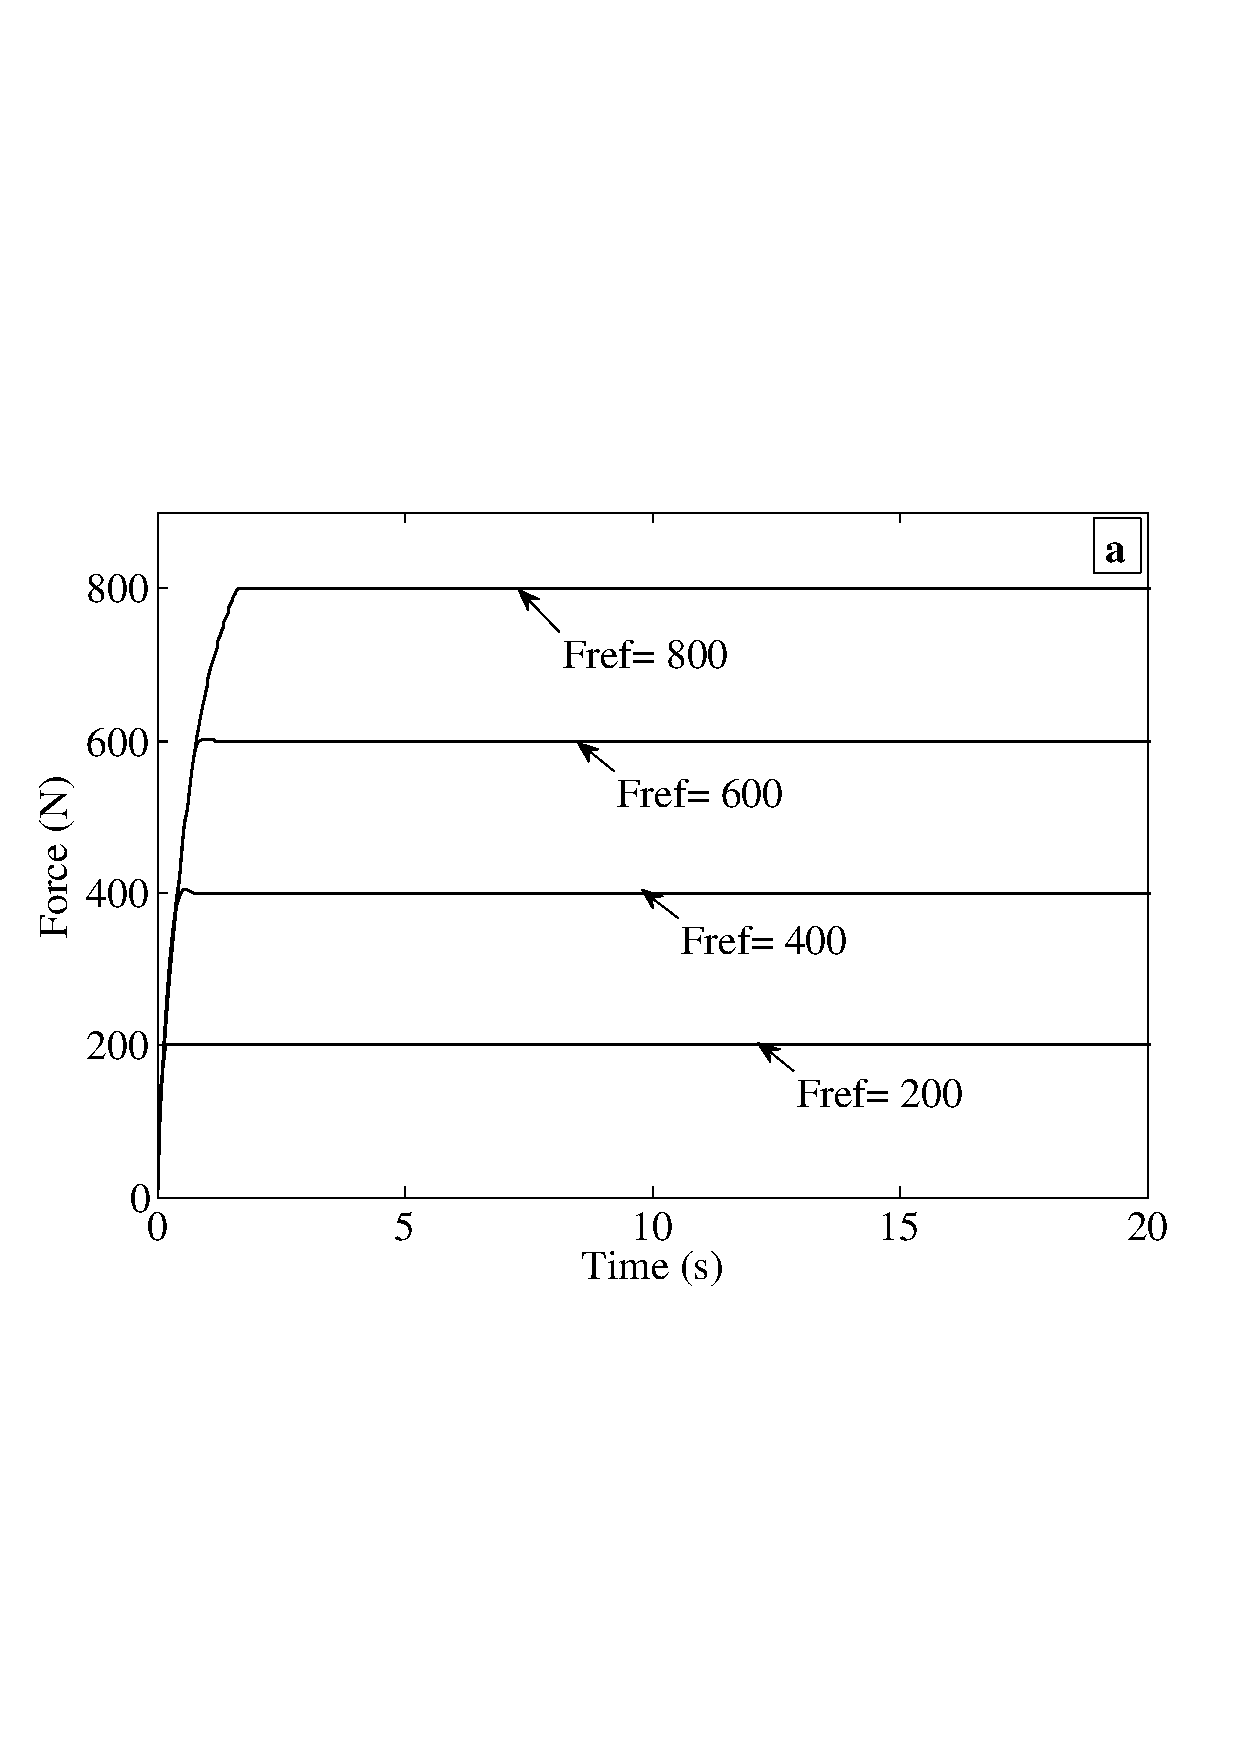
\includegraphics[width=0.48\columnwidth]{sfmin200800sfatokimoy.pdf} 
		 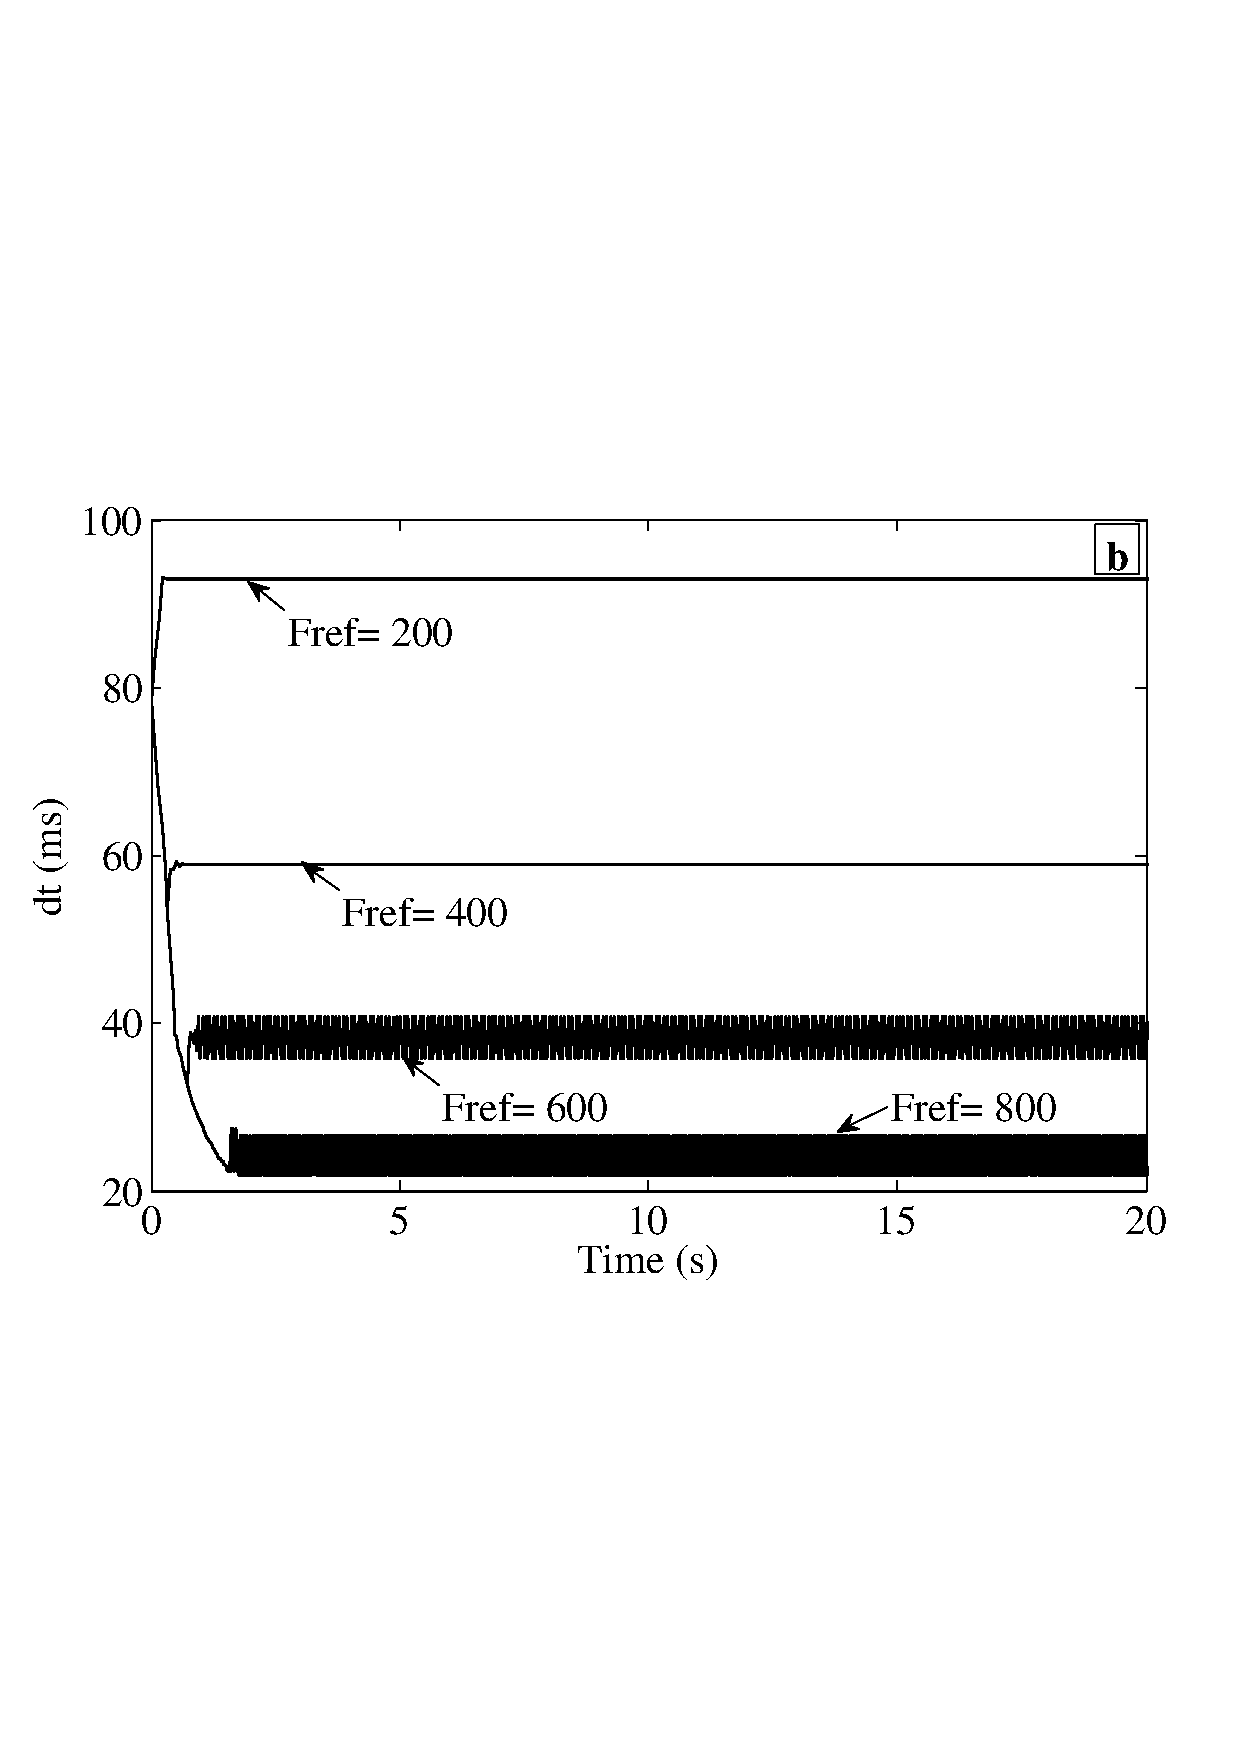
\includegraphics[width=0.48\columnwidth]{sfminsansfatdt200_800.pdf} 
		 \caption{Application of the minimization on the force model for the different reference forces $F_{ref}$= 200, 400, 600 and 800 N. (a) the developed force obtained. (b) the $dt$ corresponding to the force.}
 \end{figure}

\begin{figure}[t!]
		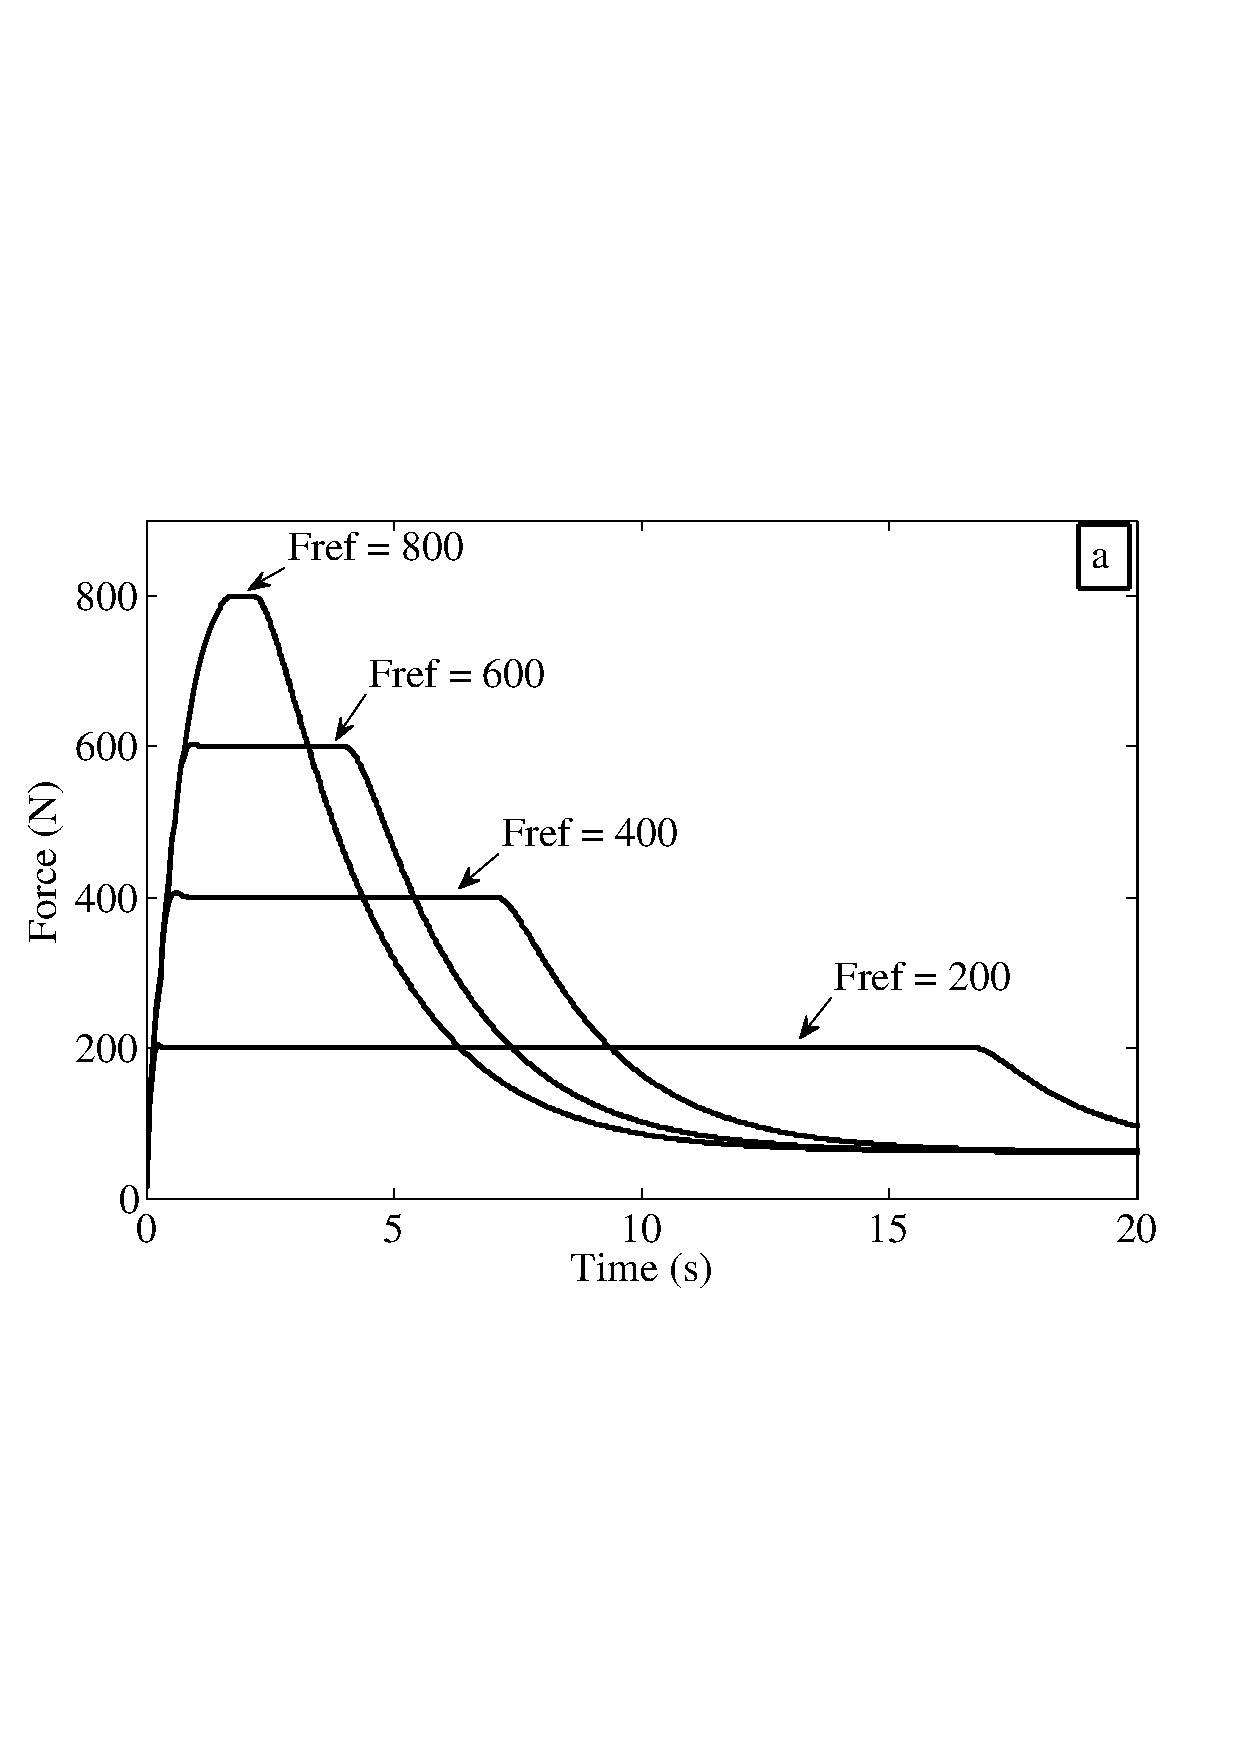
\includegraphics[width=.48\columnwidth]{fmin200800moyoki1.pdf} 
		 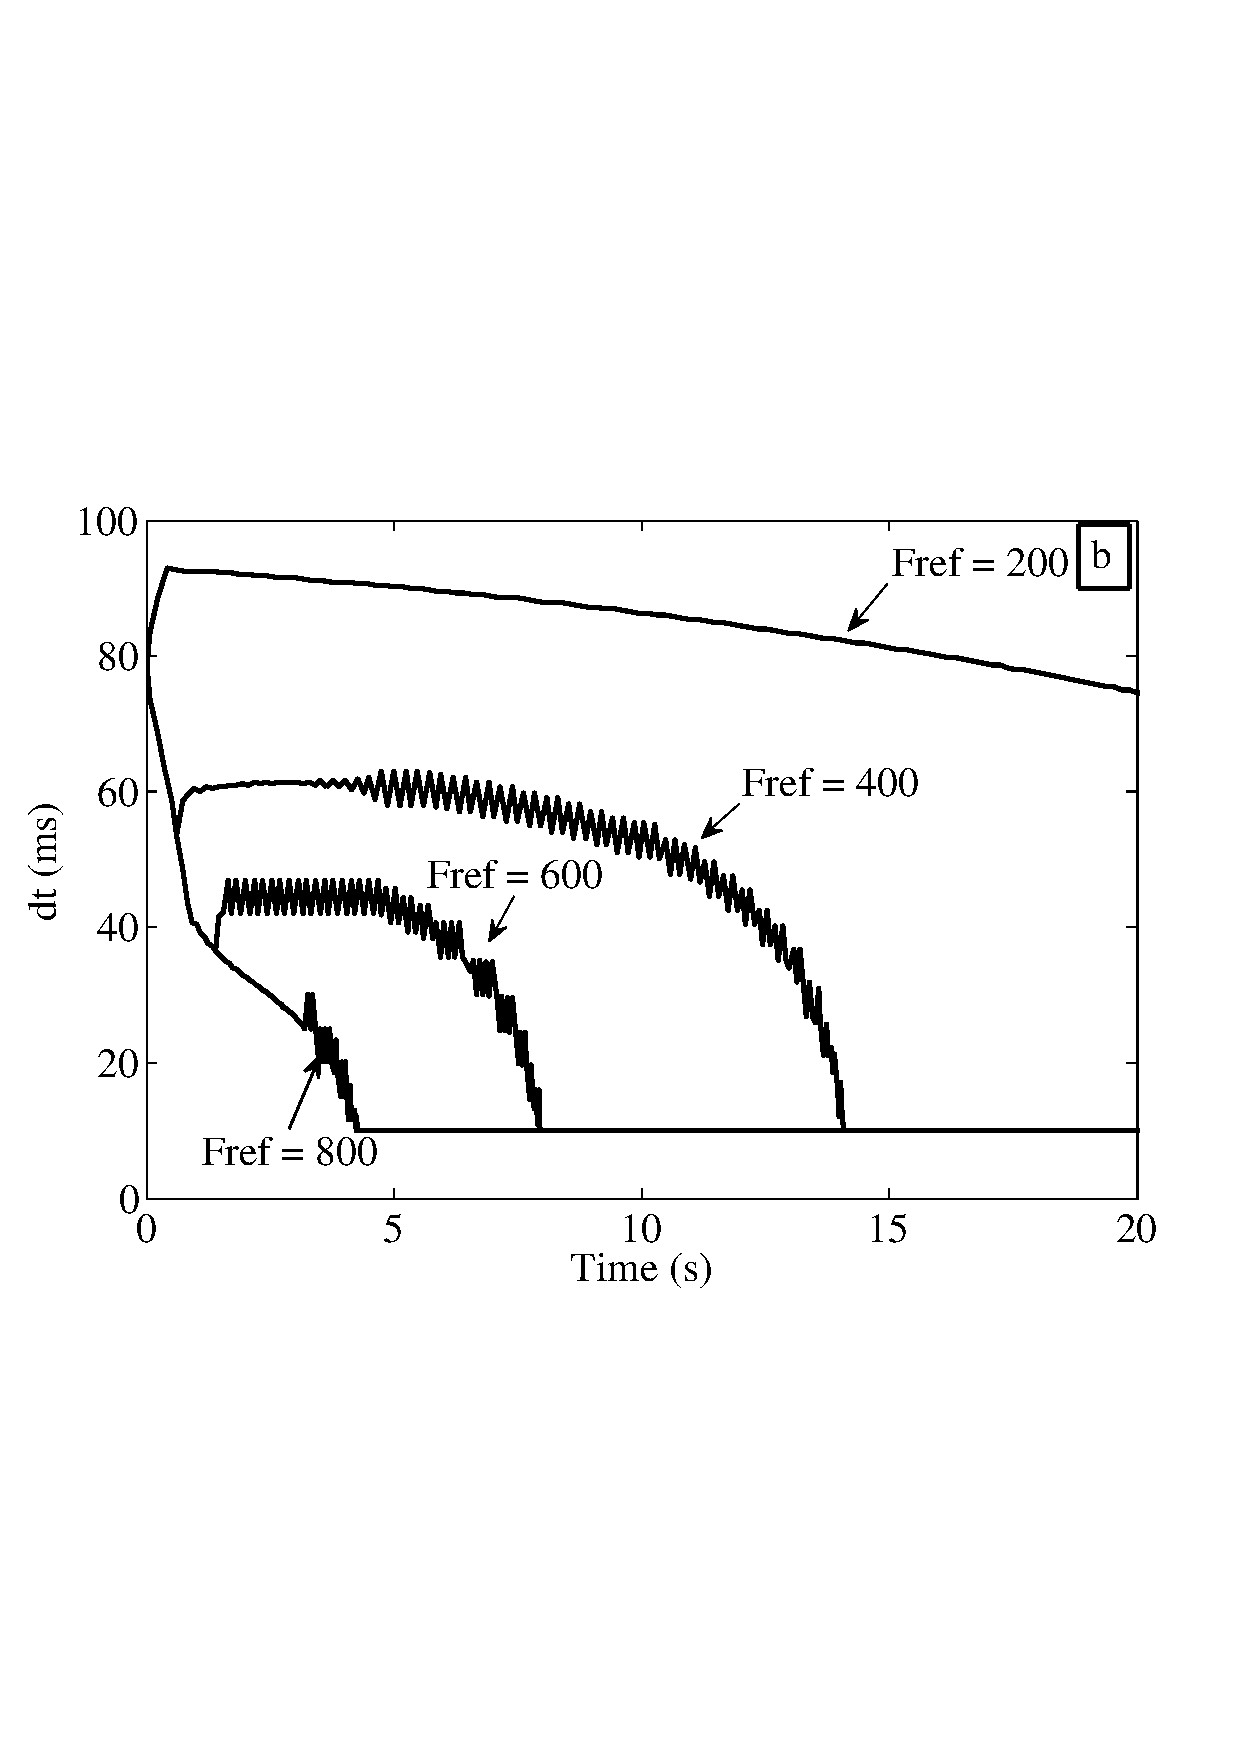
\includegraphics[width=.48\columnwidth]{dtokimini1.pdf} 
		 \caption{Application of the minimization on the fatigue model for the reference forces $F_{ref}$= 200, 400, 600 and 800 N. (a) the generated force of the model (II) and (b) the $dt$ corresponding to the force.}
		 \end{figure}  
 
\begin{figure}[b!]
	\centering
			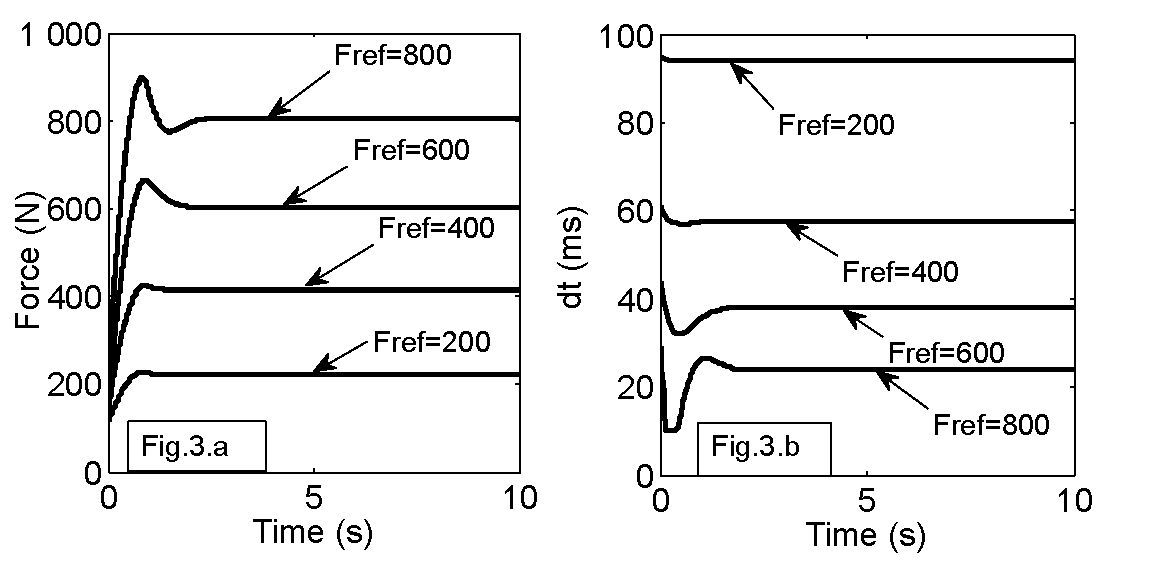
\includegraphics[width=\columnwidth]{controlpisansfatigue200_800moyeneoki.pdf}
		\caption{Effects of proportional integrator control on the model (I) without fatigue. In fig.3.a: the developed forces for four desired forces $F_{ref}$= 200, 400, 600 and 800 N. In fig.3.b: the $dt$ computed from the PI control.}
	\label{fig:controlpisansfatigue200_800moyene}
 \end{figure}

The minimization control is applied on the models (I and II) for the reference forces $F_{ref}$ equal to 200, 400, 600 and 800 N. The results of the using of the minimization on the models are shown on the figures 1 and 2. The figure 1 represents the results of the minimization on the force model with the force obtained (fig. 1(a)) and the time $dt$ corresponding (fig. 1(b)). We can observe that the generated force reach the force desired. On the figure 2 we observe the results of the application of the minimization on the fatigue model. In fig. 2(a) the developed force during the simulation with the $dt$ obtained (fig. 2(b)). We can note that the developed force reach the reference force for a certain time before to decrease due to the appearance of the muscular fatigue. The forces stabilize at the same value considered as the plateau reach. The generated force stay more longer at the desired force for a small reference than for a high. In comparing to the forces obtained for the two studies, we obtained the same values for the forces but also for the times $dt$. Contrary to the force model, the $dt$ obtained for the fatigue model decrease since a limit reach for all the $F_{ref}$.\\

The second control method applied to the models (I and II) is tested for different reference forces (200, 400, 600 and 800 N) and the results are presented in the figures 3 and 4. First, the PI control is applied on the model (I). Table I gives the $dt$ values corresponding to each $F_{ref}$. Then the found $dt$ are applied to the model (II) without the use of the PI control. The $dt$ remains constant at their found values during the simulation. Model (II) is then simulated using PI controller. The coefficients $k_p$ and $k_i$ are chosen by applying the Ziegler-Nichols method. In the figure 3, we can observe the effect of the PI control on the model (I). The PI control allows the systems to reach the mean value corresponding to $F_{ref}$ and it maintains the mean value at wanted forces by adjusting the inter pulses duration ($dt$). We can observe on figure 4 the results about model (II) with and without PI controller. In the figure 4.a the dotted curves correspond to the developed forces with the PI control and the curves in continuous line represent the developed force without control. We note that, for low values of $F_{ref}$ the force can be maintained around the mean value of $F_{ref}$ longer with the PI control than without it. The PI controller is able to reach the reference forces more quickly than without using the PI controller. This is especially visible for the high reference forces. The loss of force, induced by the appearance of muscular fatigue, is counterbalanced with the modification of $dt$ durations between each consecutive pulse which are visible in the figure 4.b.

\begin{figure}[t]
	\centering
 		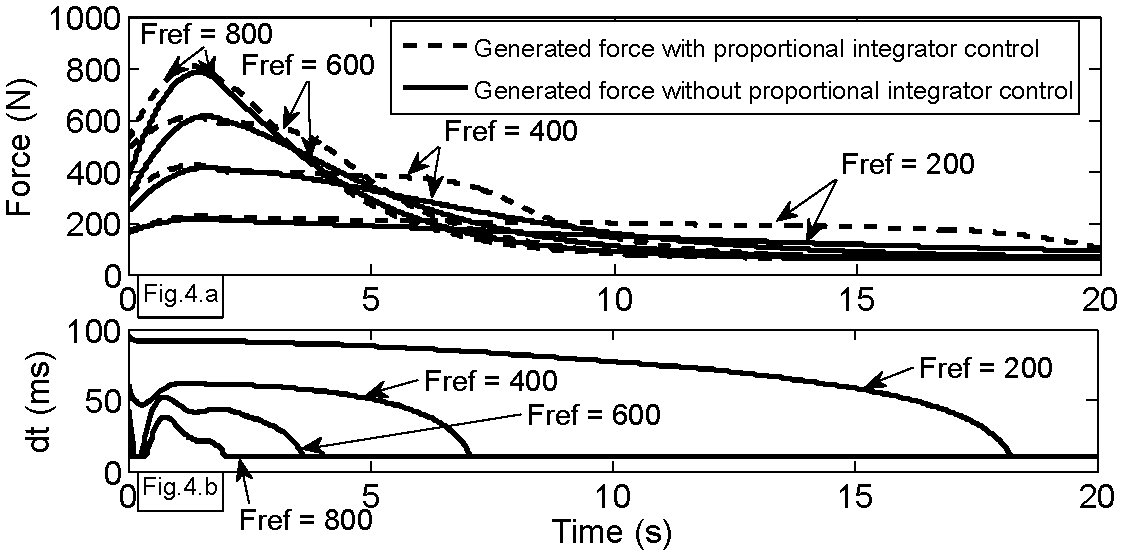
\includegraphics[width=\columnwidth]{ctrlfatiguepi200_800moyene.pdf}
 	\caption{Application of the proportional integrator control on the model (II). For four desired forces $F_{ref}$= 200, 400, 600 and 800 N , the developed forces in fig.4.a and the $dt$ computed fig.4.b .}
	\label{fig:ctrlfatiguepi200_800moyene}
	\end{figure}
	

	\begin{table}[t]
	\centering
	\caption{Table of the $dt$ corresponding in $F_{ref}$.}
		\begin{tabular}{|c|c|}
		\hline
			dt (ms) & F (N) \\
			\hline
			94.9 & 200 \\
			61.2 & 400 \\
			43.8 & 600 \\
			29.1 & 800 \\
		\hline 
		\end{tabular}
		\vspace{-0.5cm}
\end{table}

\begin{figure}[ht!]
\centering
 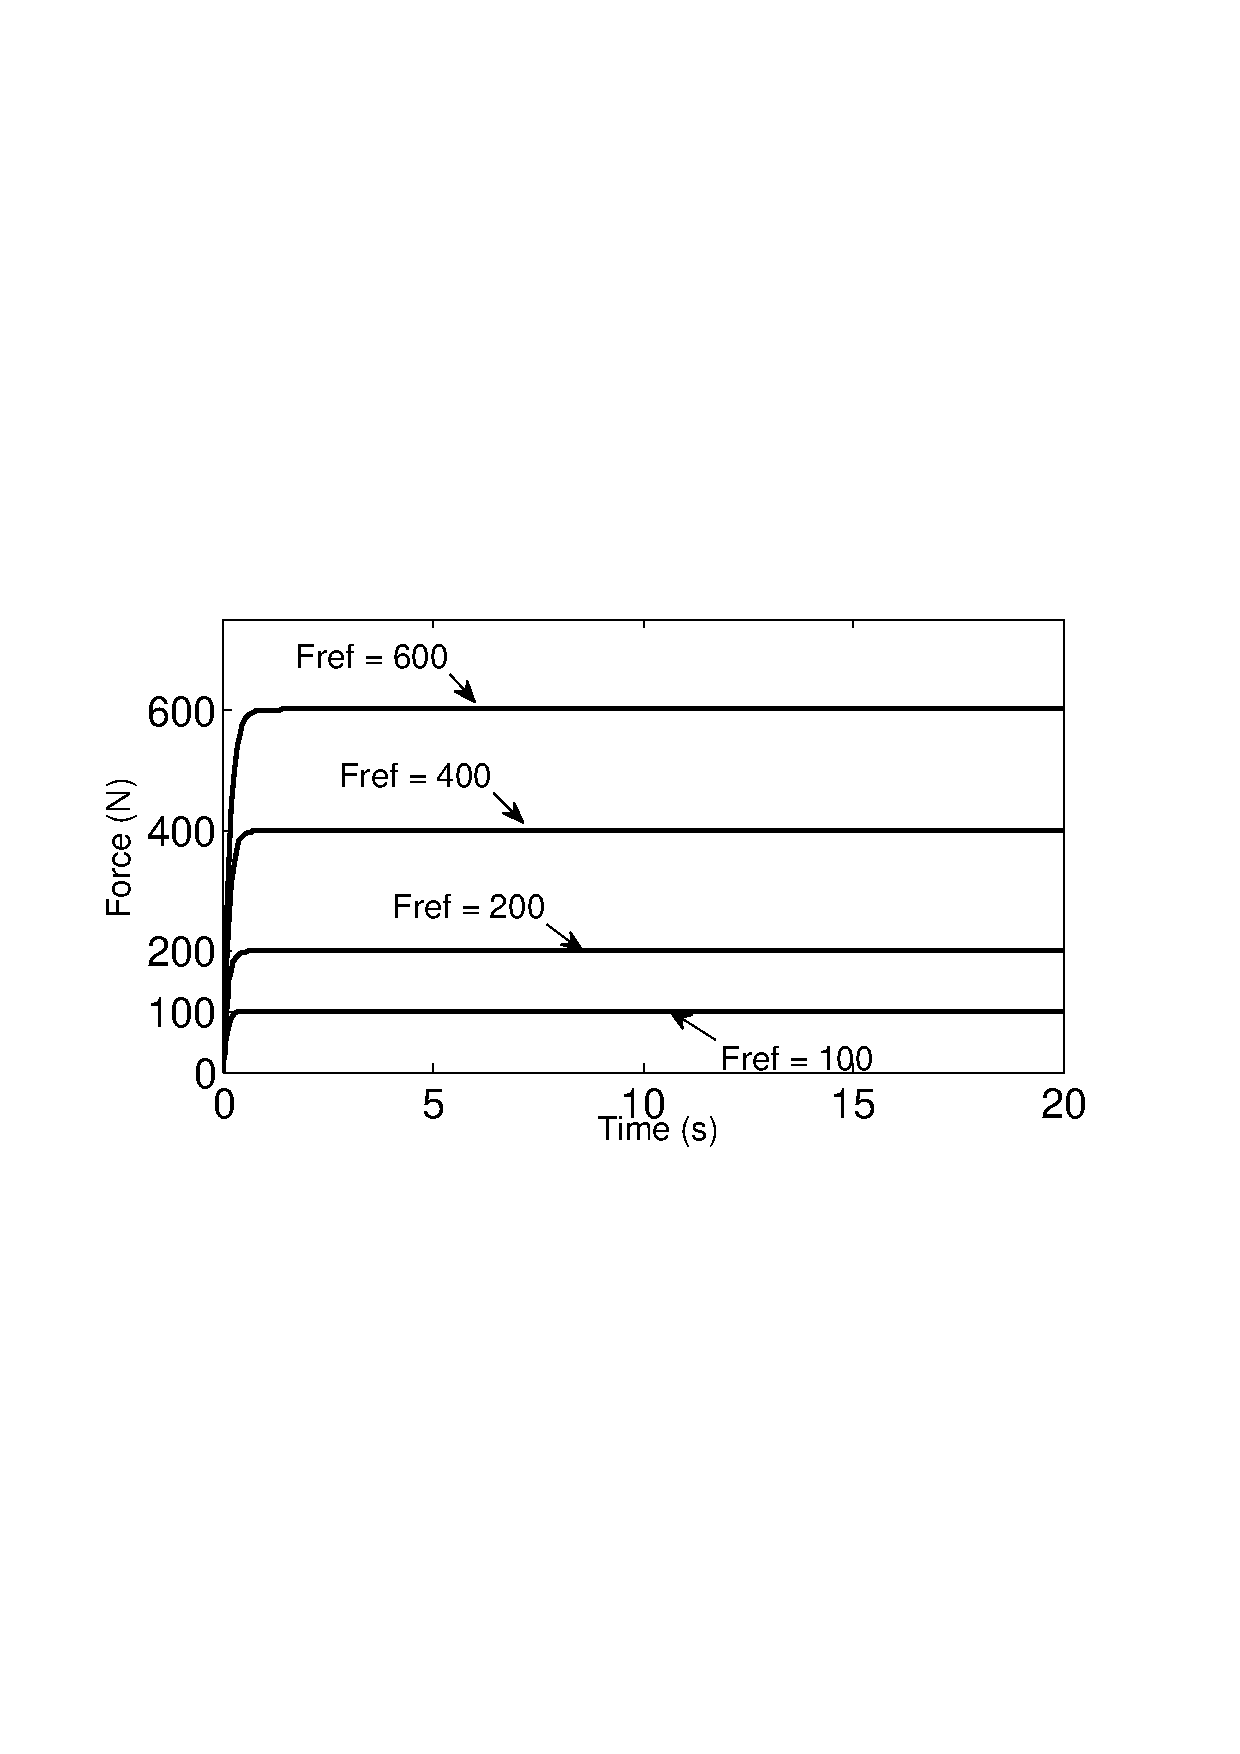
\includegraphics[width=\columnwidth]{courbes100_600uconstant.pdf}
 \caption{Results of the constant nonlinear control corresponding to $F_{ref}$ = 100, 200, 400 and 600 N.}
\end{figure}

\begin{figure}[b!]
	\centering
	\vspace{-1.8cm}
 		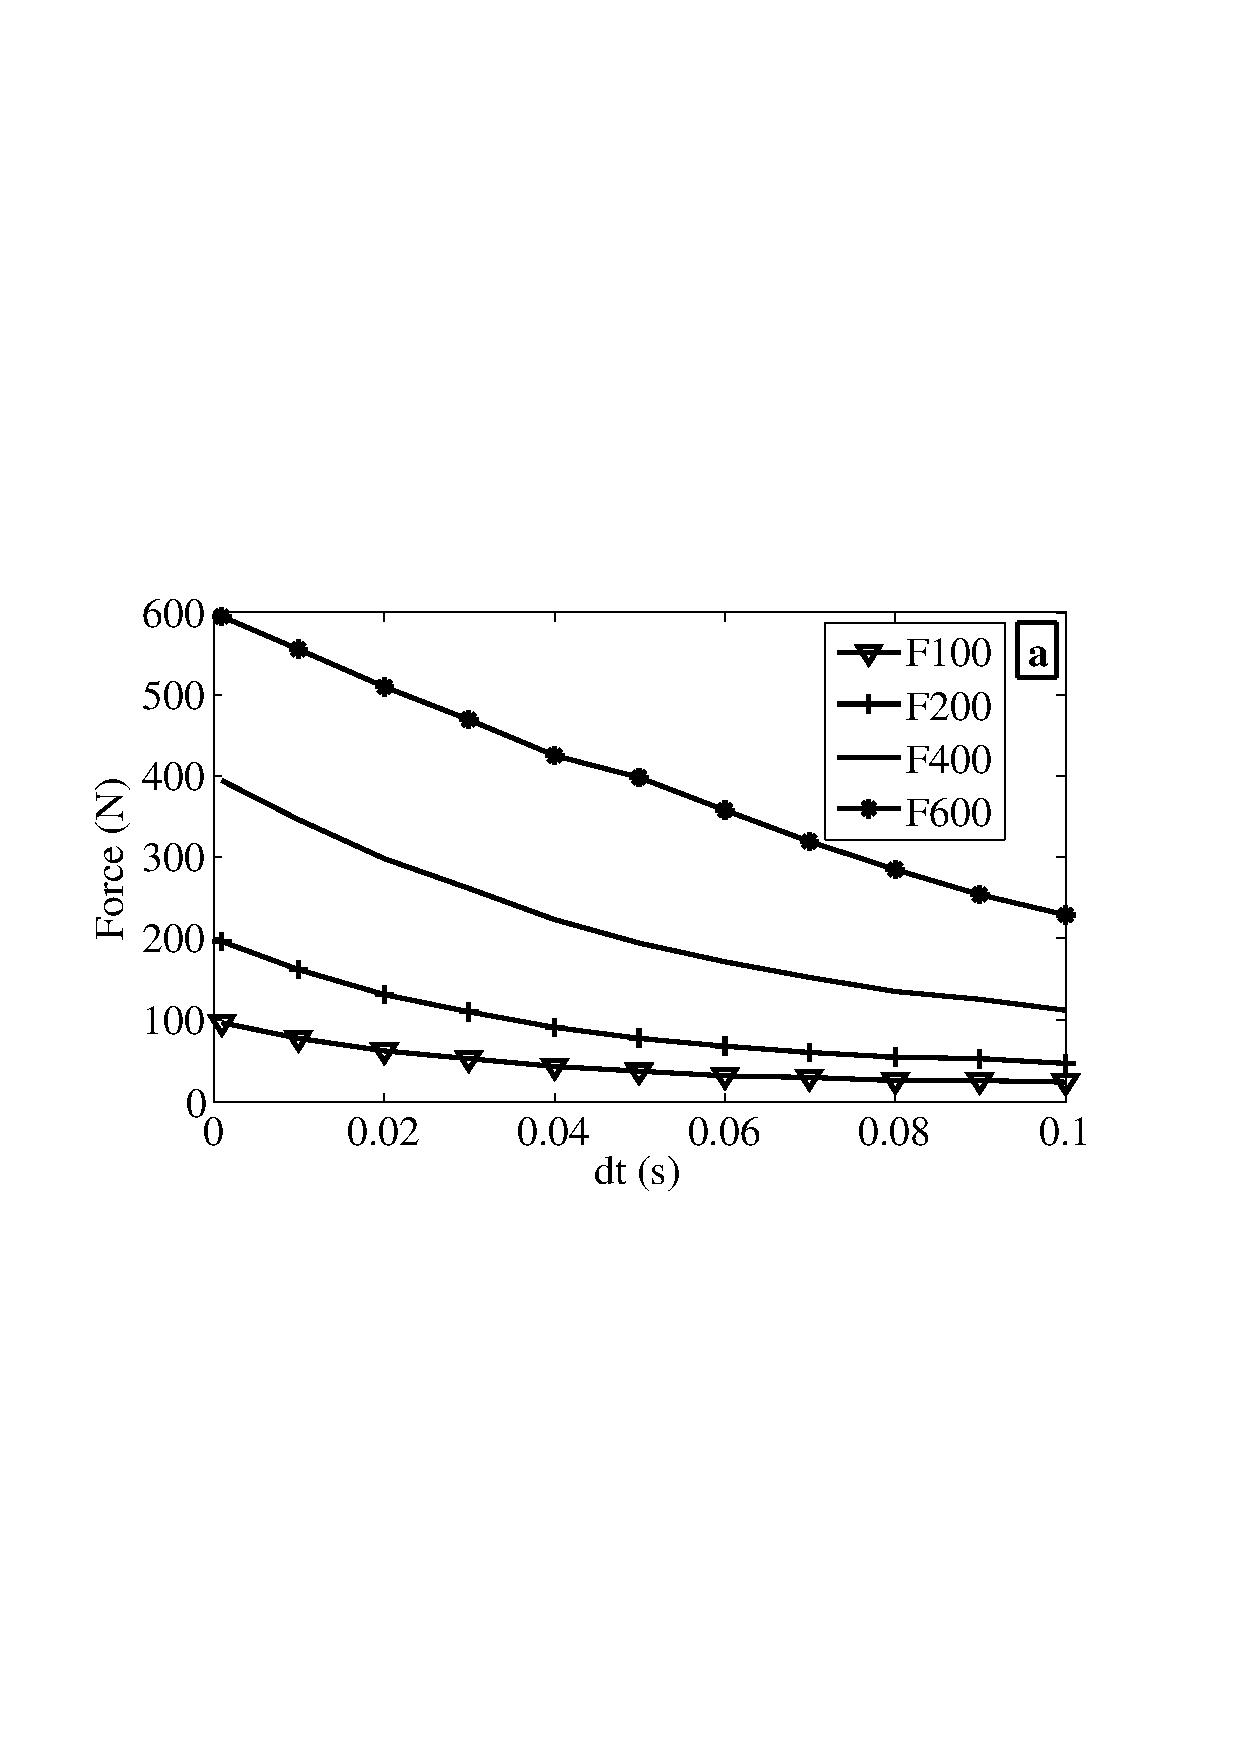
\includegraphics[width=0.48\columnwidth]{ffref_sommedessous_oki.pdf} 
		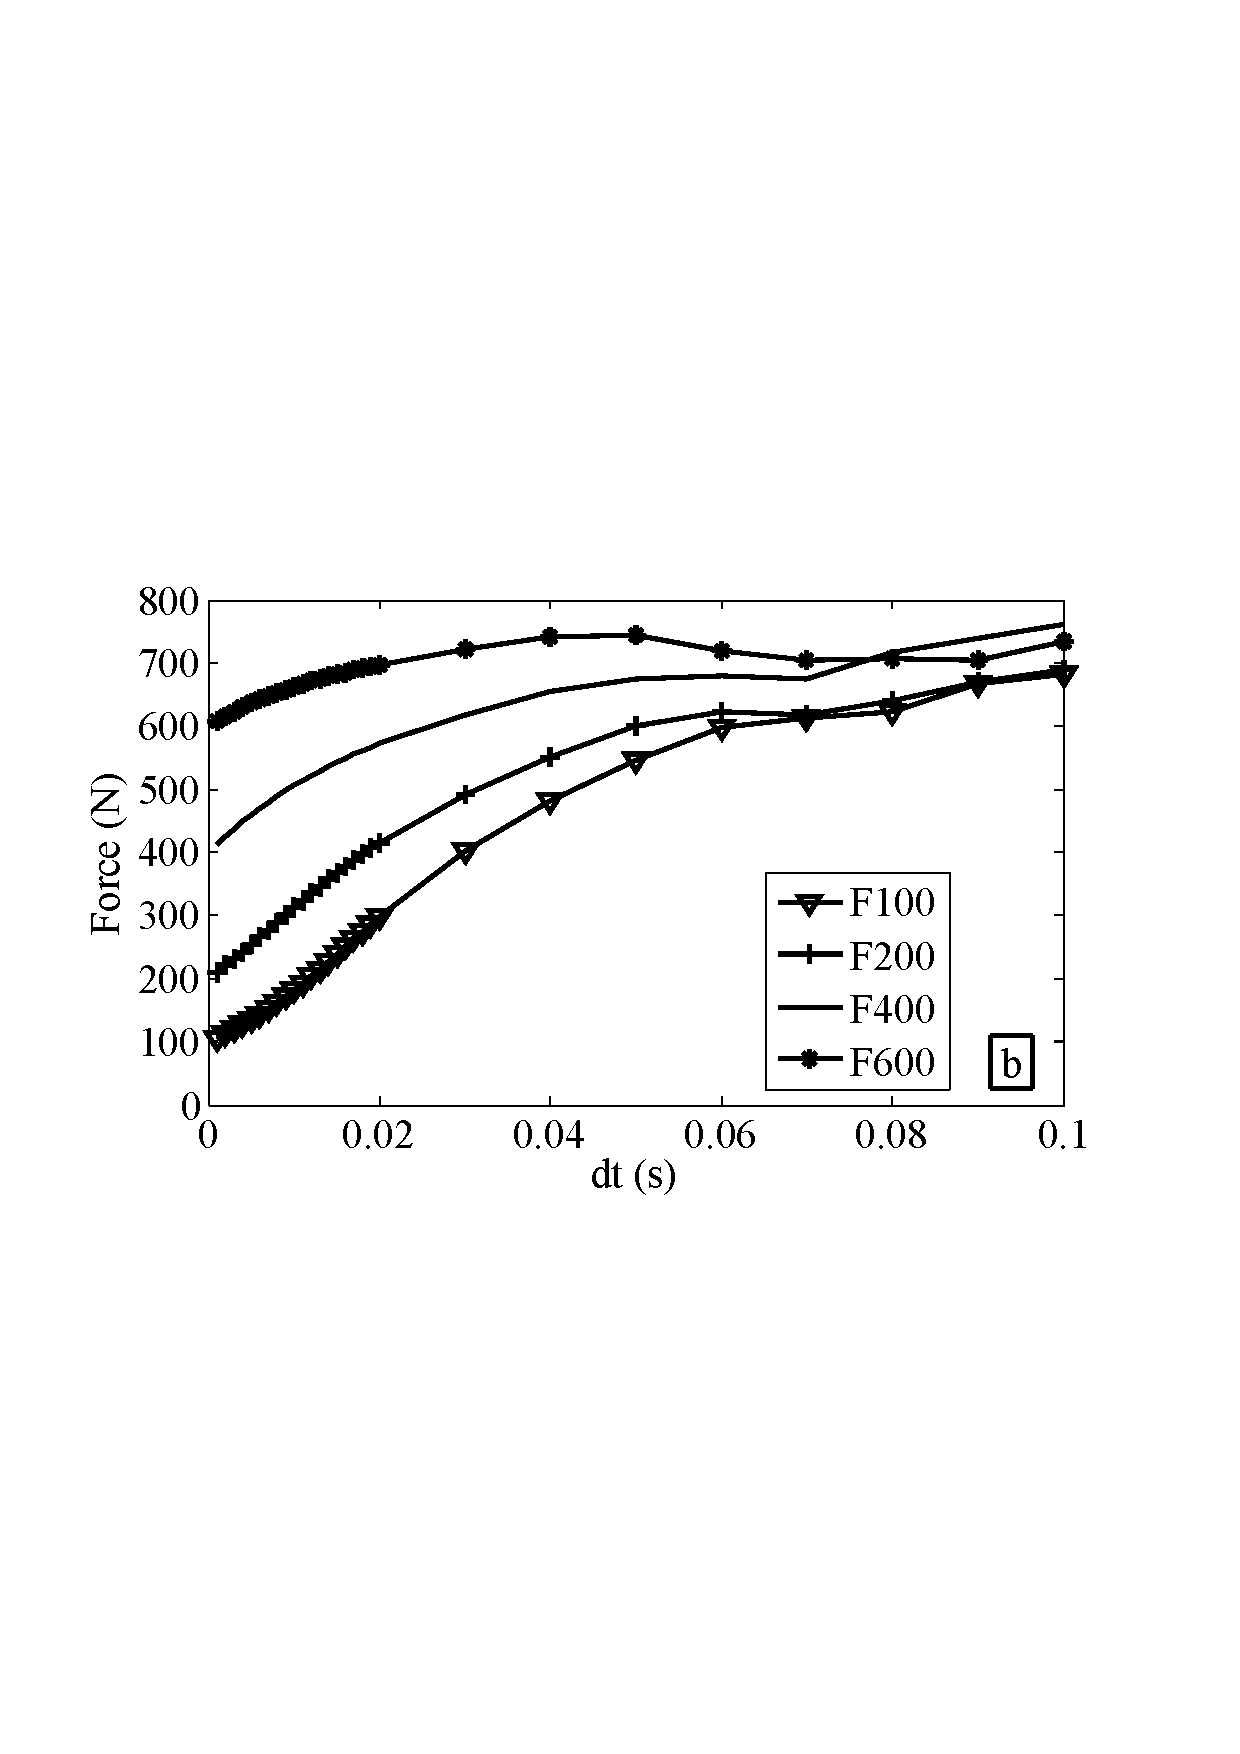
\includegraphics[width=0.48\columnwidth]{fforceoki.pdf} 
		\vspace{-1.8cm}
		\caption{Application of the nonlinear control on the force model for the two cases. Representation of the evolution of the force $F$ reached in function of the stimulation time $dt$ for the sum lower (a) and greater (b).}
 	\end{figure}
The last control method is tested for various reference forces (100, 200, 400, 600 N). The results of the nonlinear control on the model (I) are shown on the figure 5. We can observe that the generated forces reach the reference forces. At each time, the control is computed which gives the stimulation pattern to reach the reference force. The nonlinear control is applied on the models (I and II) and the results are presented in figures 6 and 7, for low values of $F_{ref}$. Different stimulation times $dt$ are fixed in the range from 1 to 100 ms. More the stimulation inter pulse time of muscle is high, more the force diverges from the reference force. The generated force with respect to $dt$ obtained for the model (I) is presented in figure 6.a in the case where the sum is lower than the nonlinear control and 6.b in the case where the sum is greater. For a short stimulation time, the force is close to the desired force. \\

The results of the application on the model (II) including the muscular fatigue are presented on the figure 7. The developed force shown in fig.7.a. is the force resulted for the sum inferior and respectively for the second case, the results are observed on the figure 7.b. As the model (I) we observe that the force is near to the wanted value for a short stimulation time. The force decreases quicker than the force model due to the parameters of the fatigue which are taken into account. We note that when the sum is superior to the nonlinear control, the force values increase and inversely in the other case the force values decrease. For the two cases, if we study the rise time to reach 90\% $F_{max}$, generally the models have needs of 0,3 s to reach 90\% of the maximal force. In the first case, the model is longer to reach 90\% of the maximal capability for a low reference contrary to the second case, where the rise time is more higher for a high reference. With the results of the nonlinear control, the study on the variation of the impulse amplitude, we observe that the force goes away of the consign when the impulse amplitude is higher. The model become unstable and uncontrollable. This phenomena is seen more quickly with the appearance of the muscular fatigue. The figure 8 allows to observe that the sum is well lower or greater than the nonlinear control. Compared with the results we can note that all the curves follow the same tendencies for the different reference forces and correspond well to the expectations.
 \begin{figure}[t!]
	\centering
	\vspace{-2cm}
		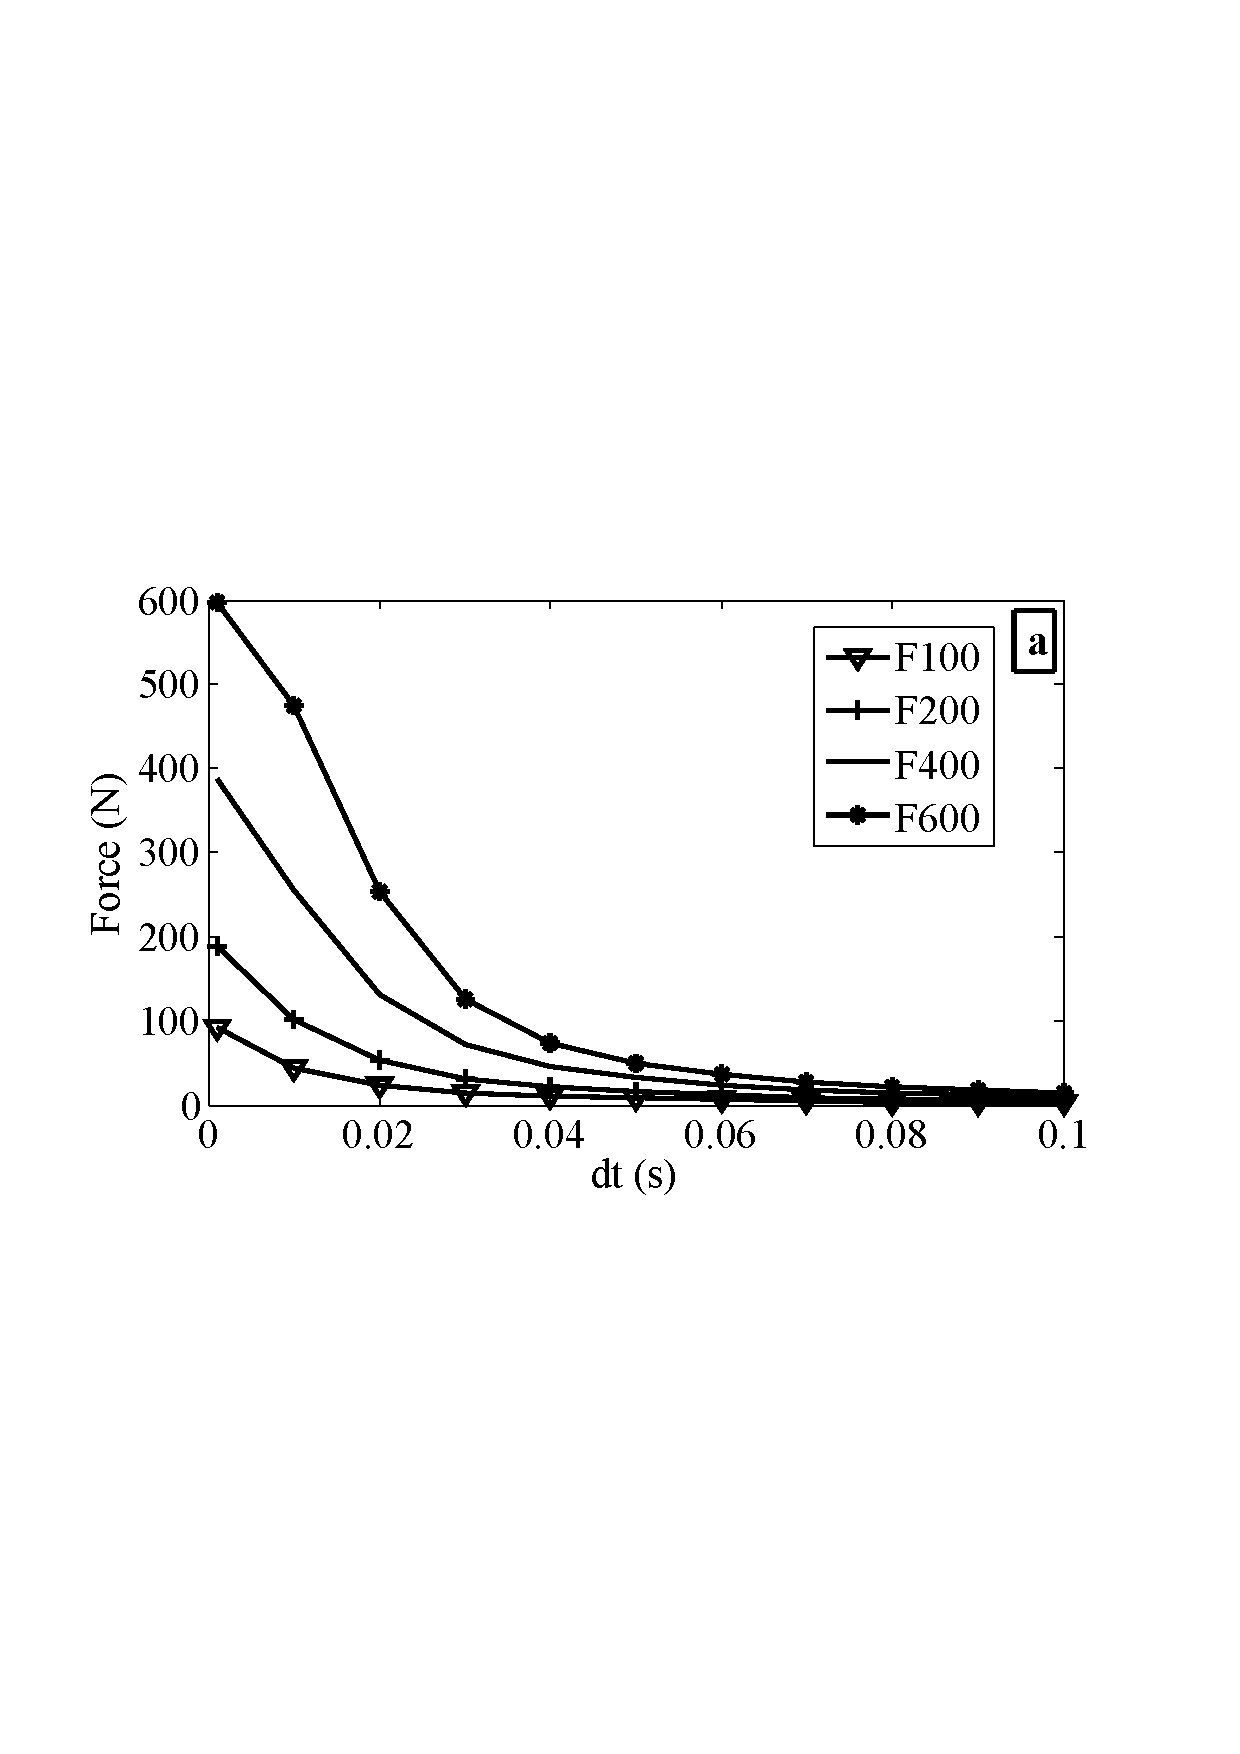
\includegraphics[width=0.48\columnwidth]{fsdessousfat.pdf}
		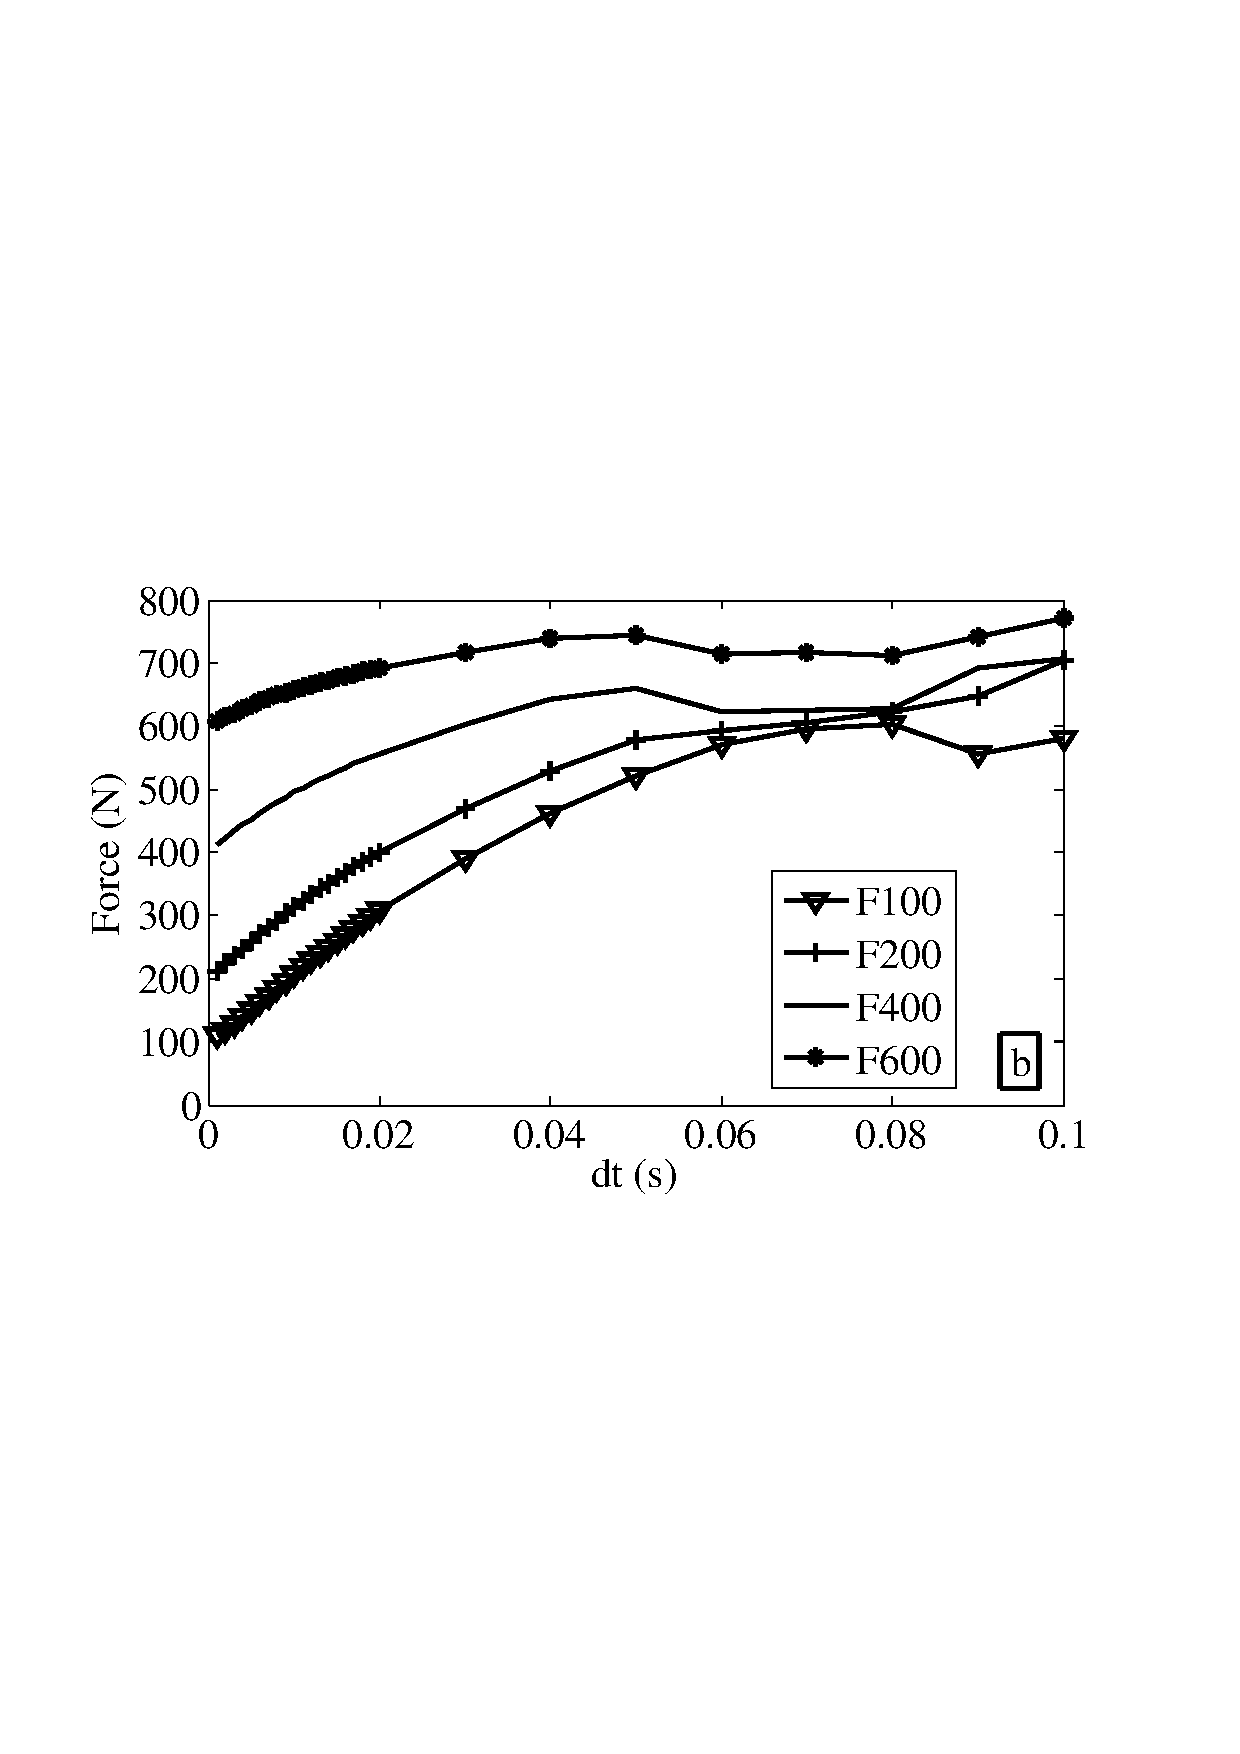
\includegraphics[width=0.48\columnwidth]{ffatoki.pdf}
		\vspace{-1.8cm}
\caption{Application of the nonlinear control on the fatigue model. Evolution of the force $F$ reached in function of the stimulation time $dt$ for the sum lower (a) and greater (b).}
\vspace{-0.5cm}
	\end{figure}
	
\section{Conclusion}

In this work, we used control methods on models (I and II) to control the force with the effects of the muscular fatigue. The minimization control, acting on the stimulation time $t_i$, maintains correctly the developed forces around a desired consign as long as possible with the influence of the muscular fatigue on the force. The proportional integrator control maintains also correctly the developed forces around a desired consign as long as possible with the influence of the muscular fatigue on the force. However, the proportional integrator control having several drawbacks, the nonlinear control has been applied on the models by acting on the amplitude variation. With regard to the simulations results obtained, we can conclude that the control methods have a good efficiency on the models. However, the models are constrained by limits to control the fatigue. In future work, we modeled the curves obtained with an optimization method, observe the errors obtained. In an other study, we apply the nonlinear control on the amplitude variation in averaged the sum of exponential. We had also add an integrator and different noises to our control method in order to be near of experimental results. Then we can test experimentally the methods. In a future study, we could compare various methods and conclude to the efficiency of our nonlinear control. 

\begin{figure}[b!]
\centering
\vspace{-0.5cm}
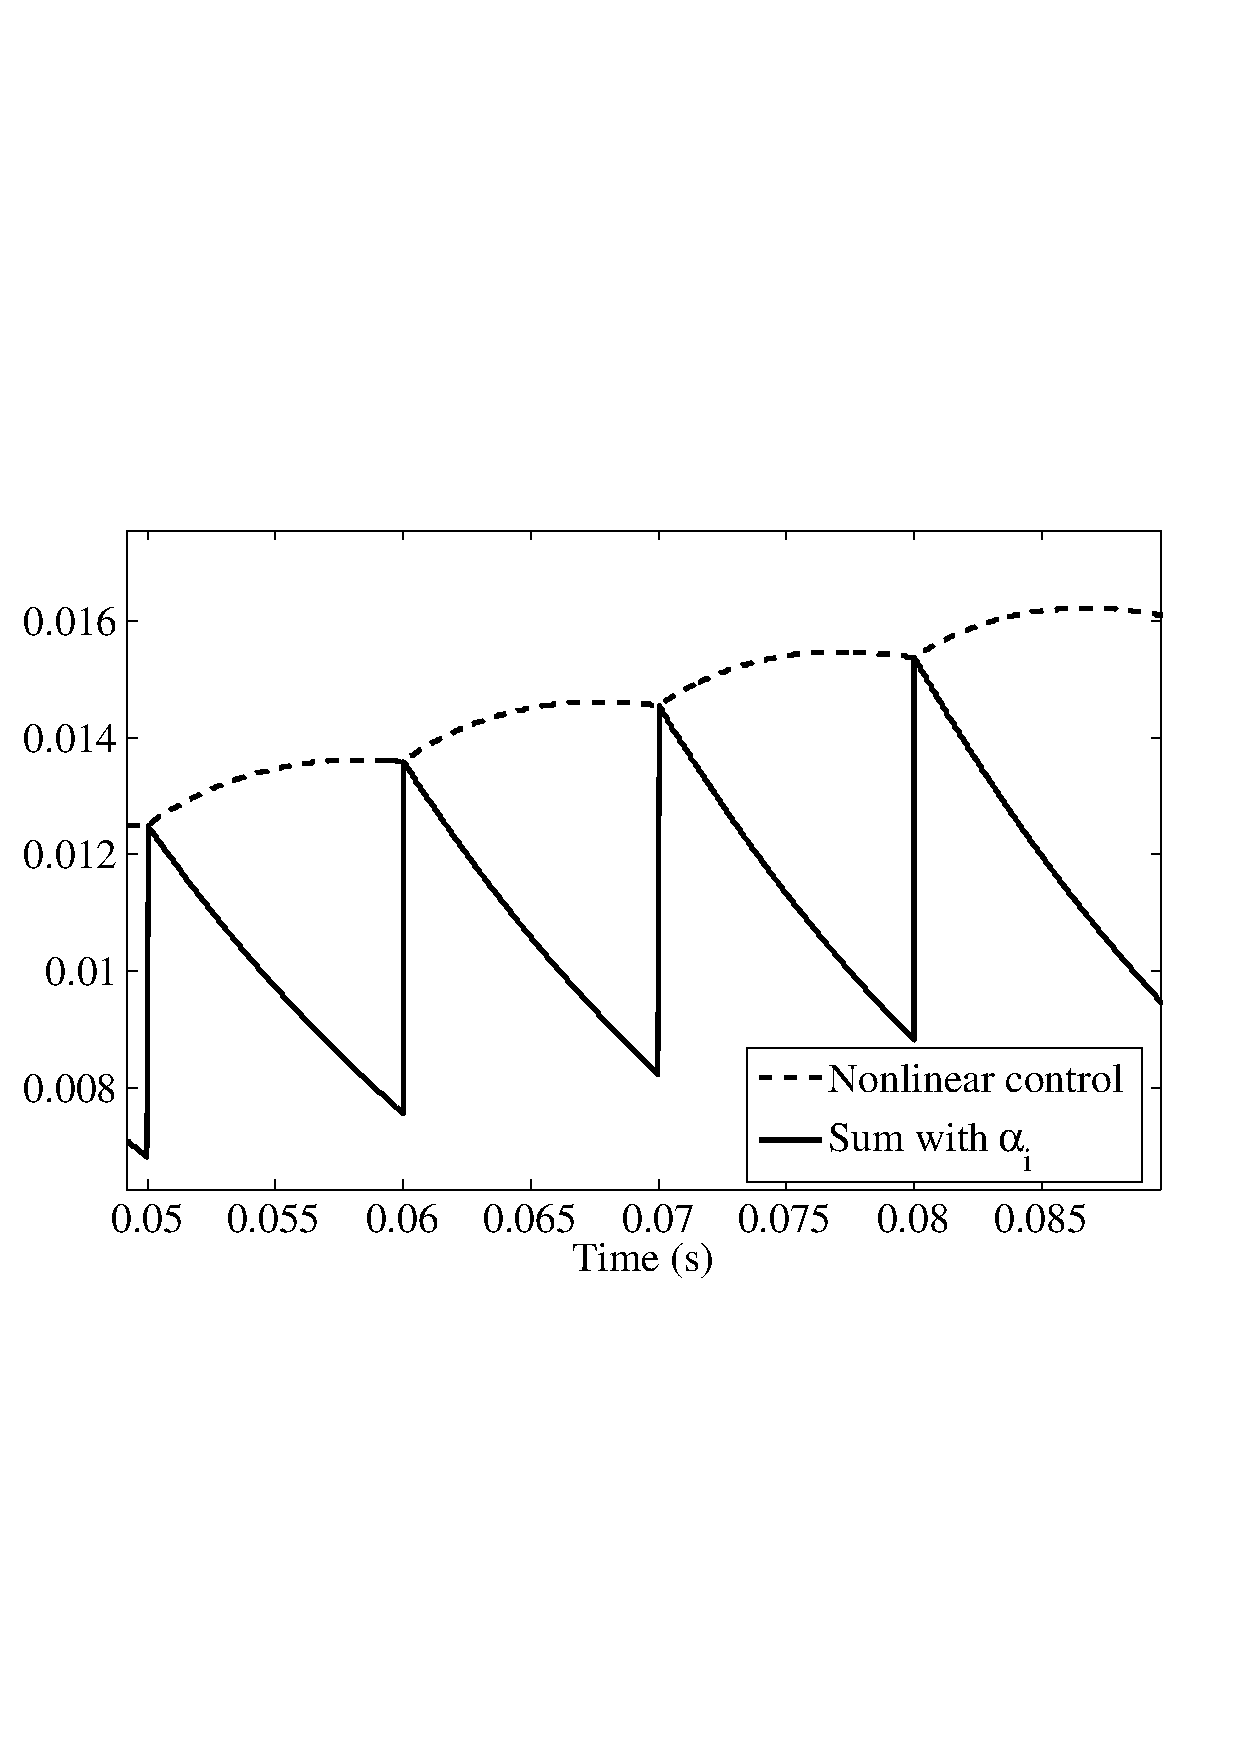
\includegraphics[width=0.48\columnwidth]{preuvesdessous1.pdf}
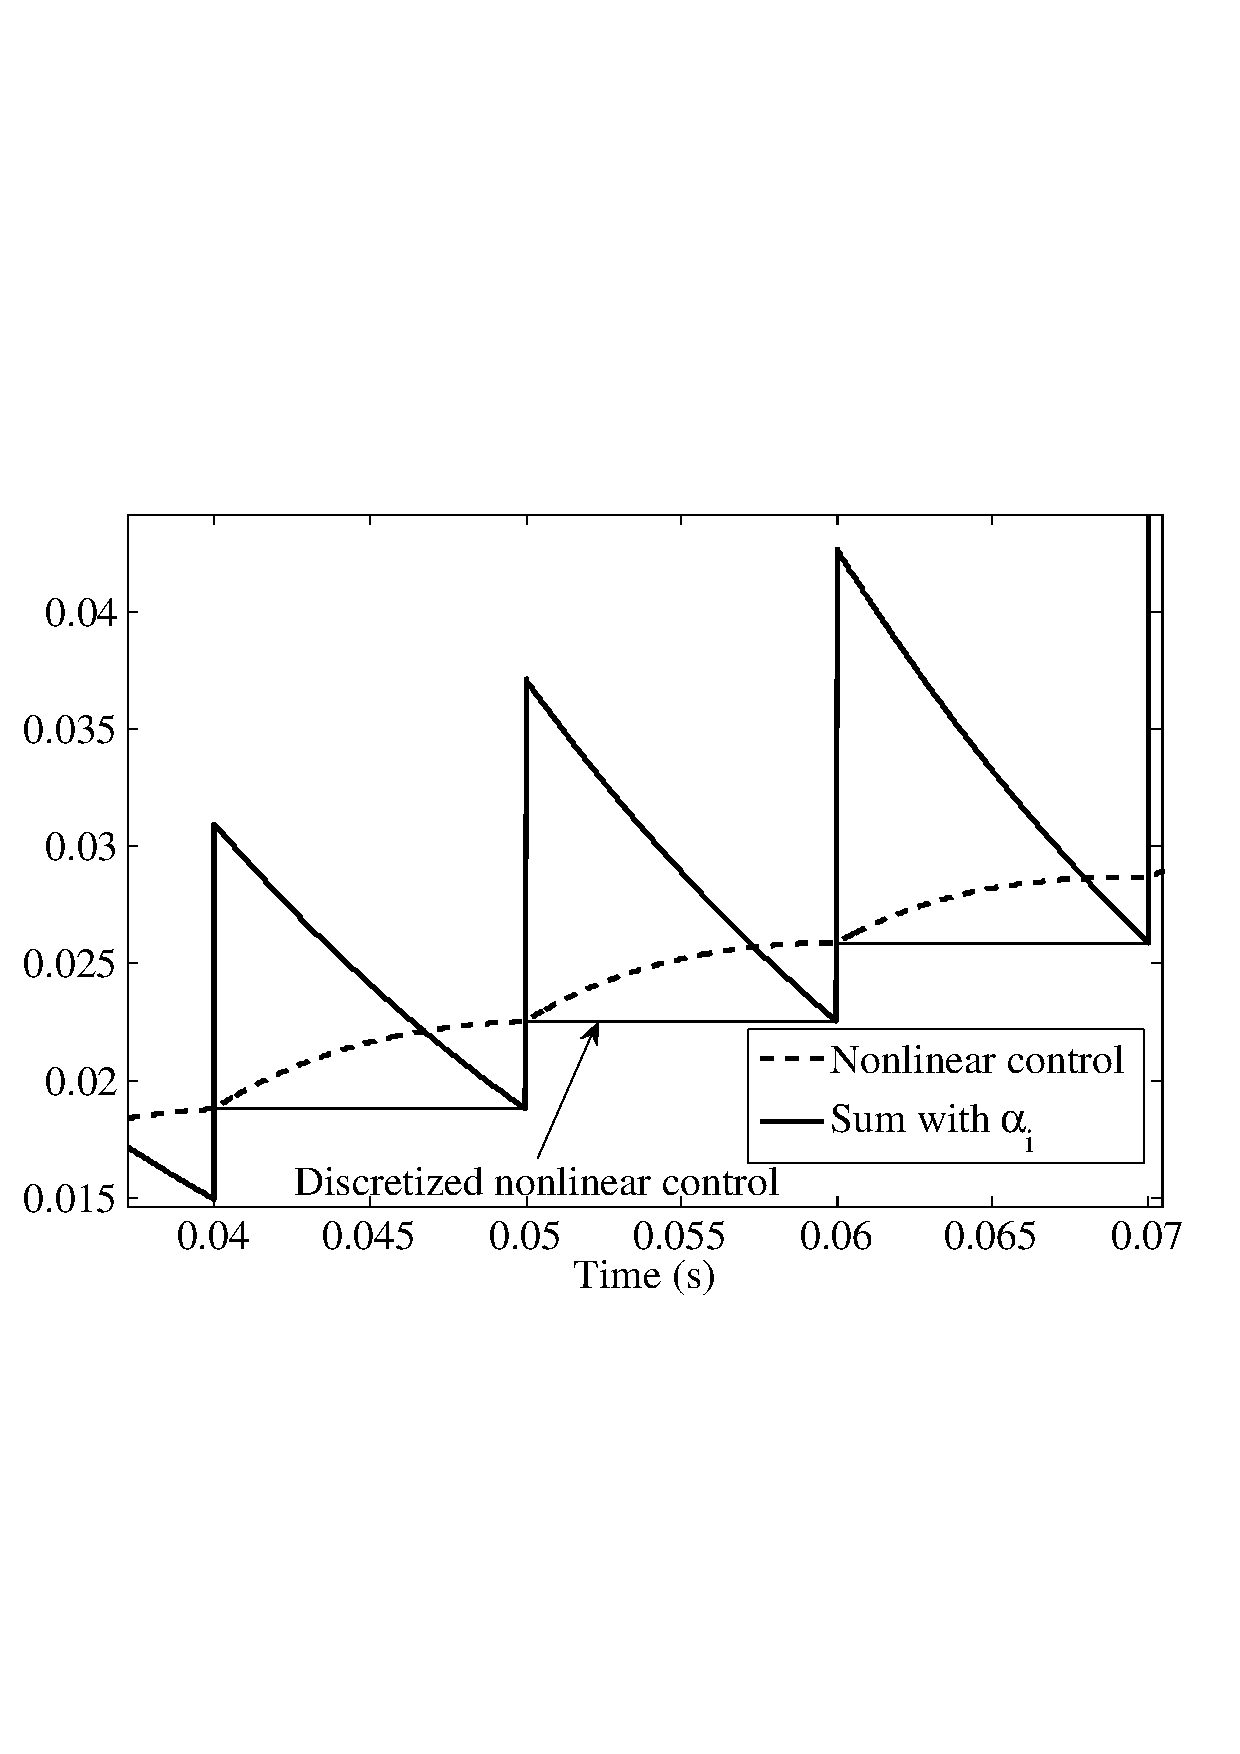
\includegraphics[width=0.48\columnwidth]{preuvesdessus1.pdf}
\caption{Representation of the two cases of sum in the nonlinear control method. To left, the representation of the sum inferior to the $u$ with to right the representation of the sum superior to $u$.}
\end{figure}

\begin{thebibliography}{1}
\small{
\bibitem{IEEEhowto:1}
Z.~Li, M.~Hayashibe, C.~Fattal and D.~Guiraud, "Muscle fatigue tracking with evoked EMG via recurrent neural network: toward personalized neuroprosthetics", IEEE Computational Intelligence Magazine, 2014, 9 (2), 38-46.
\bibitem{IEEEhowto:2}
J.~Ding, A.~S. Wexler and S.~A. Binder-Macleod, "A predictive fatigue model-I: Predicting the effect of stimulation frequency and pattern on fatigue", IEEE Transactions on Neural Systems and Rehabilitation, vol 10, no 1 March 2002.
\bibitem{IEEEhowto:3}
J.~Ding, A.~S. Wexler, and S.~A. Binder-Macleod, "A predictive fatigue model-II: Predicting the effect of resting times on fatigue", IEEE Transactions on Neural Systems and Rehabilitation, vol 10, no 1 March 2002.
\bibitem{IEEEhowto:4} 
Li-Wei Chou, Jun Ding, Anthony S. Wexler, Stuart A. Binder-Macleod, "Predicting optimal electrical stimulation for repetitive human muscle activation", International Congress Series 15 (2005) 300-309.
\bibitem{IEEEhowto:5}
 Jun Ding, Anthony S. Wexler, Stuart A. Binder-Macleod, "Mathematical models for fatigue minimization during functional electrical stimulation", International Congress Series 13 (2003) 575-588.
\bibitem{IEEEhowto:6}
Jun Ding, Stuart A. Binder-Macleod, Anthony S. Wexler, "Two-step, predictive, isometric force model tested on data from human and rat muscles", Journal of Applied Physiology 85 (1998) 2176-2189.
\bibitem{IEEEhowto:7} 
Jun Ding, Anthony S. Wexler, Stuart A. Binder-Macleod, "A mathematical model that predicts the force-frequency relationship of human skeletal muscle", Wiley Periodicals, Inc. Muscle Nerve 26 (2002) 477-485.
\bibitem{IEEEhowto:8}
 Samuel C. K. Lee, Jun Ding, Laura A. Prosser, Anthony S. Wexler, Stuart A. Binder-Macleod, "A predictive mathematical model of muscle forces for children with cerebral palsy", Developmental Medicine and Child Neurology, 2009, 51: 949-958.
}
\end{thebibliography}

	

%
%\maketitle
%%\thispagestyle{empty}
%
%\begin{abstract}
%\acresetall  % reset the acronyms from the title (if any)
%The ABSTRACT is to be in fully-justified italicized text, at the top
   %of the left-hand column, below the author and affiliation
   %information. Use the word ``Abstract'' as the title, in 12-point
   %Times, boldface type, centered relative to the column, initially
   %capitalized. The abstract is to be in 10-point, single-spaced type.
   %Leave two blank lines after the Abstract, then begin the main text.
   %Look at previous acpr abstracts to get a feel for style and length.
%\end{abstract}
%
%%% Incldue the content without .tex extension
%\acresetall  % reset the acronyms from the abstract
%\include*{content/intro/intro}          % the file wihtout .tex
%\include*{content/other/other}
%\include*{./content/acpr/example_content}
%%
%{\small
%\printbibliography
%}
\end{document}
